%We propose to use deep learning on neural networks to learn structural properties of the Internet, such as node clustering or distance between nodes. 
In this chapter, we discuss IP addresses (IPs), the unused data in internet embedding domain by illustrating (1) the reasons why IPs could reveal the structural information of  nodes in the Internet, (2) one approach  to incorporate the IPs in the internet embedding and (3)  one application which the new embedding framework can be utilized in. 

 We firstly present \system{}, a deep learning based framework to learn structural properties of the Internet, such as node clustering or distance between nodes, from the IP addresses. 
%
Existing embedding-based approaches use linear algorithms on a single source of data, such as latency or hop count information, to approximate the position of a node in the Internet.
%
In contrast, \system{} computes low-dimensional representations of nodes that preserve structural properties and non-linear relationships across multiple, heterogeneous sources of structural information, such as IP, routing, and distance information.
%
%In particular, given training data including IP address values, routing information, and hop count data, \system{} is optimized to compute low-dimensional vector representations for hosts so that both local (\eg{}, clusters of hosts) and remote (\eg{}, distances to other hosts) structural properties are well preserved.
%
Using a large real-world data set, we show that \system{} learns representations that preserve the real-world clustering of the associated nodes and predicts distance between them more than 30\% better than a mean-based approach. 
%
Furthermore, \system{} accurately imputes hop count distance to  unknown hosts (\ie{}, not used in training) given only their IP addresses and routable prefixes.
%We introduce \system{}, a neural network that computes a low-dimensional vector representation for any host in the Internet that preserves both local (\eg{}, clusters of hosts) and remote (\eg{}, distances to other hosts) structural properties. We train \system{} using . Using a large real-world data set we show that \system{} representations preserve the real-world clustering of the associated hosts and predict distance between hosts50\% better than a mean-based approach. Furthermore, we are able to compute distance to new hosts (\ie{}, not using in training) given only their IP address and only with a small loss in accuracy.
Our framework is extensible to new data sources and applicable to a wide range of problems in network monitoring and security.


Then, we consider an important topic, spoofing defense,  based on the full knowledge of the internet structural properties.  Map-based IP spoofing defenses associate source IPs to immutable structural properties of the Internet, such as paths, hop counts, or neighbors to a target, and filter out packets whose header information does not match the maps. Although accurate, existing methods lack sufficient coverage. Network maps on AS border routers do not detect spoofed packets that traverse unprotected networks. Host maps at the edge protect only against spoofed packets with source IPs known by the host. 
%
We propose to learn IP maps by constructing a structural model (or embedding) of the Internet from a limited number of measurements.  
%
We study the feasibility of learned IP maps by combining hop count filtering, a known map-based spoofing defense mechanism that maps IPs to hop counts to a target, and DIP, a deep learning based learning algorithm that computes vector representations of IPs that preserve hop count distance between them. 
%
Using a large data set of hop counts between Internet hosts, we show that learned maps can detect packets spoofed with almost {\em any} IP address and traversing {\em any} path using an embedding generated from only a few thousand IP addresses and hop counts between them.
%
In addition, our embeddings are general: an Internet model trained for a set of hosts can be used by any other host to generate new IP maps with little loss in accuracy. 

\section{Deep Learning IP Network Representations}
\subsection{Introduction}
\label{dip:intro}

The ability to map, analyze, and understand the structure of the Internet helps network management and operations by revealing opportunities for improvement or potential design flaws. For example, accurately predicting the closest server is critical in peer selection and load balancing~\citep{silkroad}. Knowing how remote IPs are clustered can help diagnose anomalous events such as spoofing attacks~\citep{hc-filter}. A holistic view of the network and its structure is essential towards achieving the  vision of self-driving networks~\citep{self-driving}. 

%The structure of a network consists of several properties such as clustering, distance, or connectivity. 
Most previous attempts to uncover the Internet structure relying on active probing from multiple vantage points using tools such as {\em traceroute} and {\em ping}~\citep{packetlab,rocketfuel}. Such techniques provide fine-grained introspection (\ie{}, can measure specific properties in specific parts of the network, such as the latency of a path) but pose a significant cost in terms of network overhead. 
%

In contrast, embedding-based approaches use fewer, strategic measurements~\citep{vivaldi,barford-sigcomm} or passive observations on network traffic~\citep{barford-imc} to learn vector representations for the network end-hosts in a low-dimensional space. The representations approximate the positions of hosts in the Internet and are used to recover structural network properties, such as distance between nodes or clustering of nodes.
%
However, the complexity of the Internet and the sparse input data make it difficult to compute accurate representations. Oftentimes, embedding approaches rely on additional data sources, which cannot be easily used in the embedding process, to refine and tune the final embeddings. For example, several embedding methods build representations based on distance-based metrics, such as latency or hop count, and then refine (or even replace) the final representations using additional probes or static information such as AS membership or routing information~\citep{vivaldi,barford-infocom}.


The emergence of deep learning as a powerful tool to extract hidden features in data calls for revisiting the problem of learning network representations through embedding. In particular, deep learning techniques provide two key benefits. First, they allow multiple heterogeneous sources of information as input, thereby identifying more accurately the relationships between multiple sources of data that jointly contribute to a specific structural property~\citep{karpathy2015deep,wang2018learning,mikolov2013exploiting}. Second, deep neuron networks are extensible and can easily incorporate additional sources of information by attaching more neurons, network layers, or network branches~\citep{wang2018learning}. One can start with a model trained on the original components and re-train it using only the newly added parts or data sources~\citep{erhan2010does}. This makes it easier for network operators to deploy, apply, or update neural network based models.


We propose \system{}, a deep learning based framework to learn the structure of the Internet. 
\system{} is a ten-layer neural network\footnote{To avoid confusion and unless explicitly stated otherwise, we use {\em network} or {\em Internet} to refer to the physical IP network and {\em neural network} to refer to the neural network we design to learn the structural properties of the physical network} that computes a low-dimensional vector representation for any node\footnote{We use {\em node} or {\em (end-)host} to denote any computer connected to the Internet and assigned an IP address.} in the Internet {\em given only its IP address and routable prefix}. \system{} preserves both local and global structure: clustered  nodes have similar representations and the distance between two representations approximates the hop count between the associated nodes.

We train our neural network using three heterogeneous data sets: hop count distances between Internet nodes, the 32 bits IP address and inter-domain routable prefix information for each node. 
%
A key insight to train \system{} is to {\em first compute representations based on the IP and routing information}, thereby recovering structural information hidden in the IP values, and refine them using a distance-based optimization.
%
As the size of the routable prefix varies by IP, we first normalize the IP and prefix data by representing an IPv4 address on 64, rather than, 32 bits. To capture structural information encoded in the IP address value, we feed the eight bytes of the normalized IP sequentially at each of the first eight layers of the neural network. We then use the last two layers to get the hop count matrix and optimize the embedding distance prediction. With a trained \system{}, we can estimate distance between {\em any} two Internet hosts as long as we have their IPs, even if they are not part of the training data. 

Results on large real-world data sets of hop counts between thousands of IP addresses and 95 geographically distributed servers show that we can predict hop count distance between known hosts (\ie{}, whose IP address were used in the training) with an absolute error of around 2 hops and over 30\% better than a mean-based method. We infer the distance between unknown IPs (\ie{}, not appearing in training data) with a small loss in accuracy compared to known IPs. In addition, the representations learned by \system{} preserve the real-world clustering of the associated hosts. The accuracy of our model increases when we increase the training data set.





%Deep learning provides both a general and an extensible framework to recover and analyze network structure from IP information and sparse distance data. \system can be easily extended to incorporate other sources of structural information, such as AS membership or latency measurements between hosts. We believe 

While our results are preliminary, they offer us a glimpse of the power of deep learning in recovering structural properties of the Internet from sparse data. \system{} is the first framework that can estimate accurately the distance to any Internet host given only its IP address and routable prefix without any distance data.
%To the best of our knowledge, this is the first attempt to learn Internet structural properties from IP address values. While our results are preliminary, they suggest the power of deep learning in identifying hidden features encoded in the value of an IP address



\subsection{Background and Related Work}
\label{dip:background}

\textbf{What is structure?} Many properties can make up the structure of the Internet: connectivity between IPs, routers, or networks; distance-based metrics such as hop count or latency; similarity-based metrics such as the set of one's neighbors in the connectivity graph; path-based properties such as the sequence of routers on a path. Here, we focus on two specific properties that define both the local and the global structure of a network: clustering of end-hosts and hop count based distance between end-hosts. %In Section, we discuss how to extend our approach to other properties.

\textbf{Network coordinate systems} learn vector representations for participating nodes such that the position of the node in the embedding approximates its position in the Internet. Most coordinate systems build embeddings using a single source of structural data: latency measurements among nodes or to predetermined landmark servers~\citep{vivaldi, gnp, pic,pyxida,zhao2011efficient} or hop count information from passive traffic observations~\citep{barford-sigcomm,barford-infocom}. 
%
Latency and hop count data is often sparse and cannot always be accurately embedded in metric spaces. To overcome these issues, several approaches use out-of-band information, such as location~\citep{vivaldi} or routing~\citep{barford-infocom} data, or perform active measurements~\citep{barford-sigcomm} to impute the missing data and detect clusters or distances.
%Because of the sparsity and structulatencies or hop counts cannot be accurately embedded in a metric space, some coordinate systems use location information to tune the embedding~\citep{vivaldi}. In contrast, we propose to train an embedding model using multiple diverse sources of data, including routing and distance information.
%
%Eriksson \etal{} use hop count information from passive traffic observations to build an embedding of the Internet~\citep{barford-infocom}. The hop count represents the number of routers on a path. Similarly to embedding-based approaches, hop count information alone is not sufficient to accurately embed all hosts. The authors resort to active probes~\citep{barford-sigcomm} or AS information~\citep{barford-infocom} to fill in missing hop count data and detect node clusters or distances. 
Unlike them, we propose to train our embedding jointly using distances, routing information and host IP values, thereby learning hidden structural features encoded in a node's IPv4 address. With a trained model, we are able to embed and find the hop count to any IP, without the participation of its host.% \mingda{and able to embed any IP address in IPv4}.

\begin{figure*}[t]
	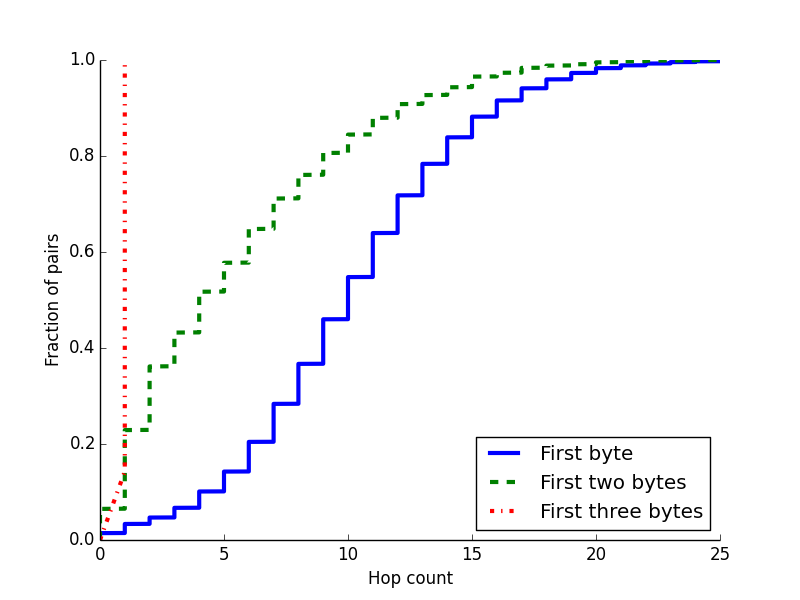
\includegraphics[width=.45\linewidth]{Graph/dip/hopcountbybyte.png}
	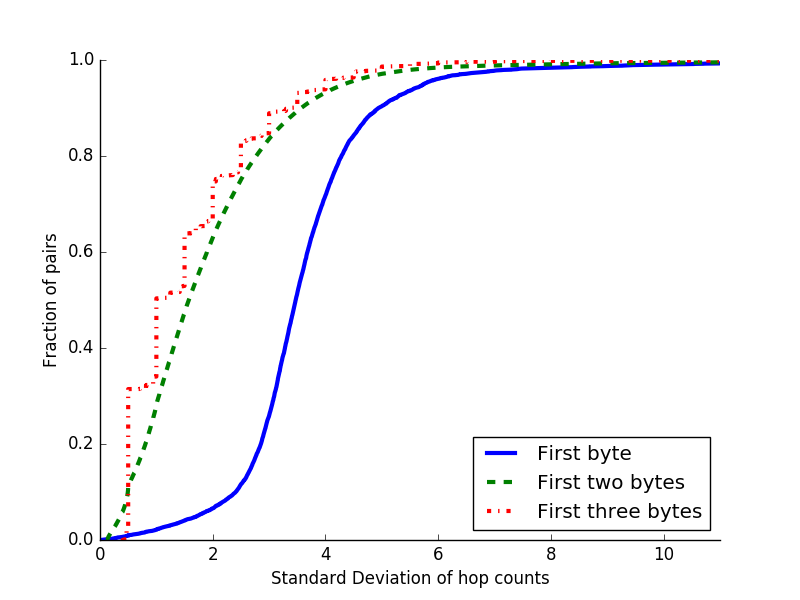
\includegraphics[width=.45\linewidth]{Graph/dip/hopcountSDbyprefix.png}
	\caption{Cumulative distribution of (left) hop counts between pairs of host-server IPs that share the first, first two, or first three bytes, and (right) standard deviation of hop count distribution among groups of IPs sharing the first, first two, or first three bytes. The more similar two IPs are, the closer they are and the more similar their distances to the same third IP are.}
	\label{fig:difference}
\end{figure*}


\textbf{Deep neural networks} consist of multiple layers of interconnected neurons~\citep{lecun2015deep}. A neuron aggregates multiple input values using local weights and biases, applies an activation function, and produces one or more numerical values as output. 
%
Given a training task, one can define an objective function to evaluate the output of the entire neural network, \eg{}, prediction error. 
%
Using gradient-based back-propagation algorithms to optimize the objective function~\citep{kingma2014adam}, neural networks automatically tune the weights and biases of each neuron to achieve a better performance.

%output by passingis a function that takes learning} generally refers to the modeling and training methods for a category of machine learning models called deep neural networks~\citep{lecun2015deep}. Informally, a deep neural network consists of multiple layers of interconnected neurons. Each neuron is a pre-defined function which takes the output from the other neruons it links with as the input, and produces one or multiple numerical values as the output. In addition, neurons control their way to aggregate the input by model parameters that are numerical values associated with links. Given training data from a specific task, one can define an objective function that evaluates the output quality of a deep neural network (\eg, prediction error). By leveraging gradient-based backpropagation algorithms~\citep{kingma2014adam} to optimize the objective function (\eg, minimize prediction error), model parameters in a deep neural network are automatically and iteratively tuned in order to achieve better performance.

%We envision deep learning as a key technique for learning structural properties of the Internet. First, the expressiveness of deep neural networks suggests they could handle the complex and non-linear structural features of the Internet. Second, neural networks are strong in learning from heterogenous data sources~\citep{karpathy2015deep,wang2018learning,mikolov2013exploiting}. This is important in the context of Internet embedding, as many structural properties can be extracted only by jointly modeling multiple data sources. For example, the value of an IP address can be combined with routing information to determine clusters of IPs. Finally, the extensibility of deep neural networks makes it easy to manage new data sources~\citep{wang2018learning} or perform incremental training~\citep{erhan2010does}.

%We vision that deep learning is the key technique that opens the door to the next generation of Internet embedding. First, based on the universal approximation theorem~\citep{csaji2001approximation}, the expressiveness of deep neural networks suggests the possibility of handling non-linear and potentially complex embedding space for Internet. Second, Internet embedding learning needs the capability of jointly modeling heterogeneous data sources. Deep neural networks are strong at learning from heterogenous data sources, and have brought great progress in challenging tasks, such as image captioning (from image to natural language)~\citep{karpathy2015deep}, image search (from natural language to image)~\citep{wang2018learning}, and machine translation (between different languages)~\citep{mikolov2013exploiting}. In the context of Internet embedding, we have realized the importance and benefit brought by the redundancy across heterogenous data sources. While a framework that is capable of synthesizing hetergeneous data into uniform representations is desired for Internet embedding, we believe that deep neural networks could be the best candidate at this moment.
%Last but not the least, the extensibility of deep neural networks makes it easy to manage heterogeneous data sources. When a new data source is added or an existing data source needs to be removed, one can add or delete a network branch~\citep{wang2018learning}, without changing the rest. In terms of incremental training, one has the flexibility to take the existing components as ``pre-trained''~\citep{erhan2010does}, and only train the newly added component. As we are able to modularize deep neural networks, it will be easier for system admins to manage data sources and update the underlying models.



\subsection{Learning Network Representations}
\label{dip:design}


%We first describe the data sources used in the learning process, and then present the neural network design for learning IP network representations.

\system{} learns an embedding model that accurately reflects the structure of the Internet, \ie{}, preserves node clustering and distances between nodes. The goal of learning is to minimize the prediction error for the distance between any two nodes. The learned model is defined by the structure of the neural network and the final values for the weights and biases of each neuron. Next, we describe the data used in learning and how we construct the neural network.

\subsubsection{Data Sources} 

%Our goal is to learn a network model that accurately reflects the structure of the Internet, \ie{}, preserves node clustering and distances between nodes. Next we identify and analyze several data sources that determine local and global structure properties.

\textbf{IP addresses and routing information.}
The IP address of a host provides a coarse indication of the location of the host in the Internet. To make routing scalable and fast, IP addresses are assigned hierarchically and divided into a  network (or routable) part and a host (or local) part. 
The routable part, usually expressed by an integer representing the number of bits (also called prefix), tells routers how to route the packet through the core of the Internet towards the destination network. Intuitively, IPs with the same routable prefix share a path towards them through the Internet core and are more likely to be close to each other.

\textbf{Hop counts.} The hop count between two hosts represents the number of routers on the default path between hosts. We use hop count, rather than latency, to measure the distance between two hosts, as it can be easily extracted from the TTL value of a network packet~\citep{hc-filter}, without active measurements. In Section~\ref{dip:discussion}, we discuss how to extend the model using latency measurements. Our hop count matrix is asymmetric and very sparse; it does not contain hop counts between all IPs. %This makes our goal more challenging as we need to deal with sparse information in learning an accurate embedding.



\subsubsection{IP Transformation}
\label{dip:ipnorm}

The key idea of our work is to use both local (IPs and routing information) and global (hop counts) structural information to guide the embedding of network nodes. By utilizing deep learning for embedding, we can identify and use hidden features encoded in the IP address of a given node. We perform several transformations on the input, guided by observations on real network data.

\textbf{IP normalization.} Because the routable information is tied to an IP address, we combine the IP and prefix values when feeding them to the neural network. To keep the size of the input constant and independent on the prefix size, we generate a {\em normalized IP address} for each regular IP. The process of normalization is depicted in Figure~\ref{fig:normalizedip}. We divide each IP into the network and the host parts. We pad the end of the network part and the beginning of the host part with zero to obtain two four-byte values. We concatenate the values and get the eight bytes normalized IP. Further, for easier processing, we represent each byte of the input in one-hot vector format (256 dimensions), \eg{}, a one and the rest are 0s, where the 1's position is the value of the byte (0 to 255).

\textbf{Sequential feeding.}  IP addresses are assigned hierarchically and encode structural information of the network. To better understand how the hierarchical assignment affects node clustering, we perform two experiments on a data set of hop counts between 95 geographically distributed servers and ten million IP addresses of end hosts. Section~\ref{subsec:data} describes the data in more detail.

First, we group all pairs of host-server IPs according to whether they share (within the pair) the first byte, first two bytes, or first three bytes. We show the all-to-all hop counts between pairs in each of the three groups in Figure~\ref{fig:difference}(left). The more similar two IP addresses are, the closer they are in terms of number of hops. 
%
Second, we group separately hosts and servers according to whether they share the first one, two, or three bytes and generate the hop count distribution for each pair of host-server groups that share the same prefix. We present the standard deviation for each pair in 
Figure~\ref{fig:difference}(right). The smaller the standard deviation is, the more similar the distances are. This means that the more similar two IPs are, the more likely they have the same hop count to another node. 






\begin{figure}
	\begin{center}
	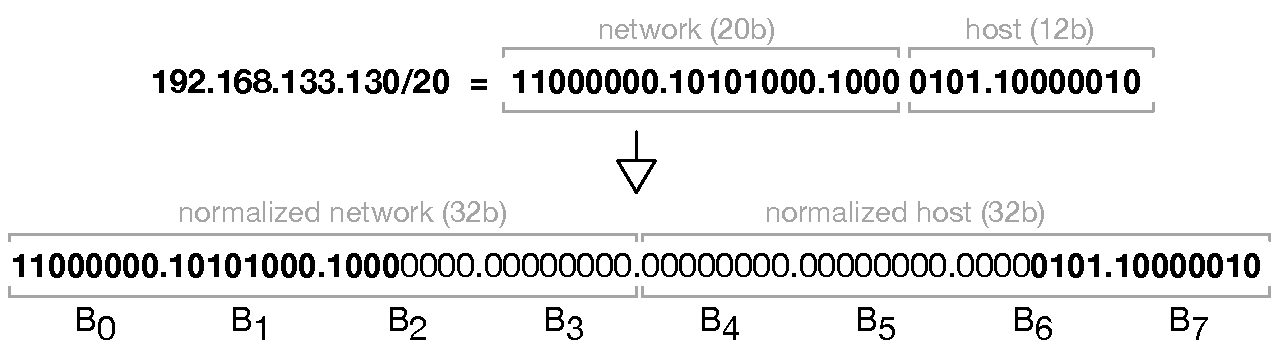
\includegraphics[width=.8\linewidth]{Graph/dip/normalized-ip}
		\end{center}
	\caption{Generating a normalized IP address for 192.168.133.130/20.}
	\label{fig:normalizedip}
\end{figure}

\begin{figure*}[t]
	\begin{center}
			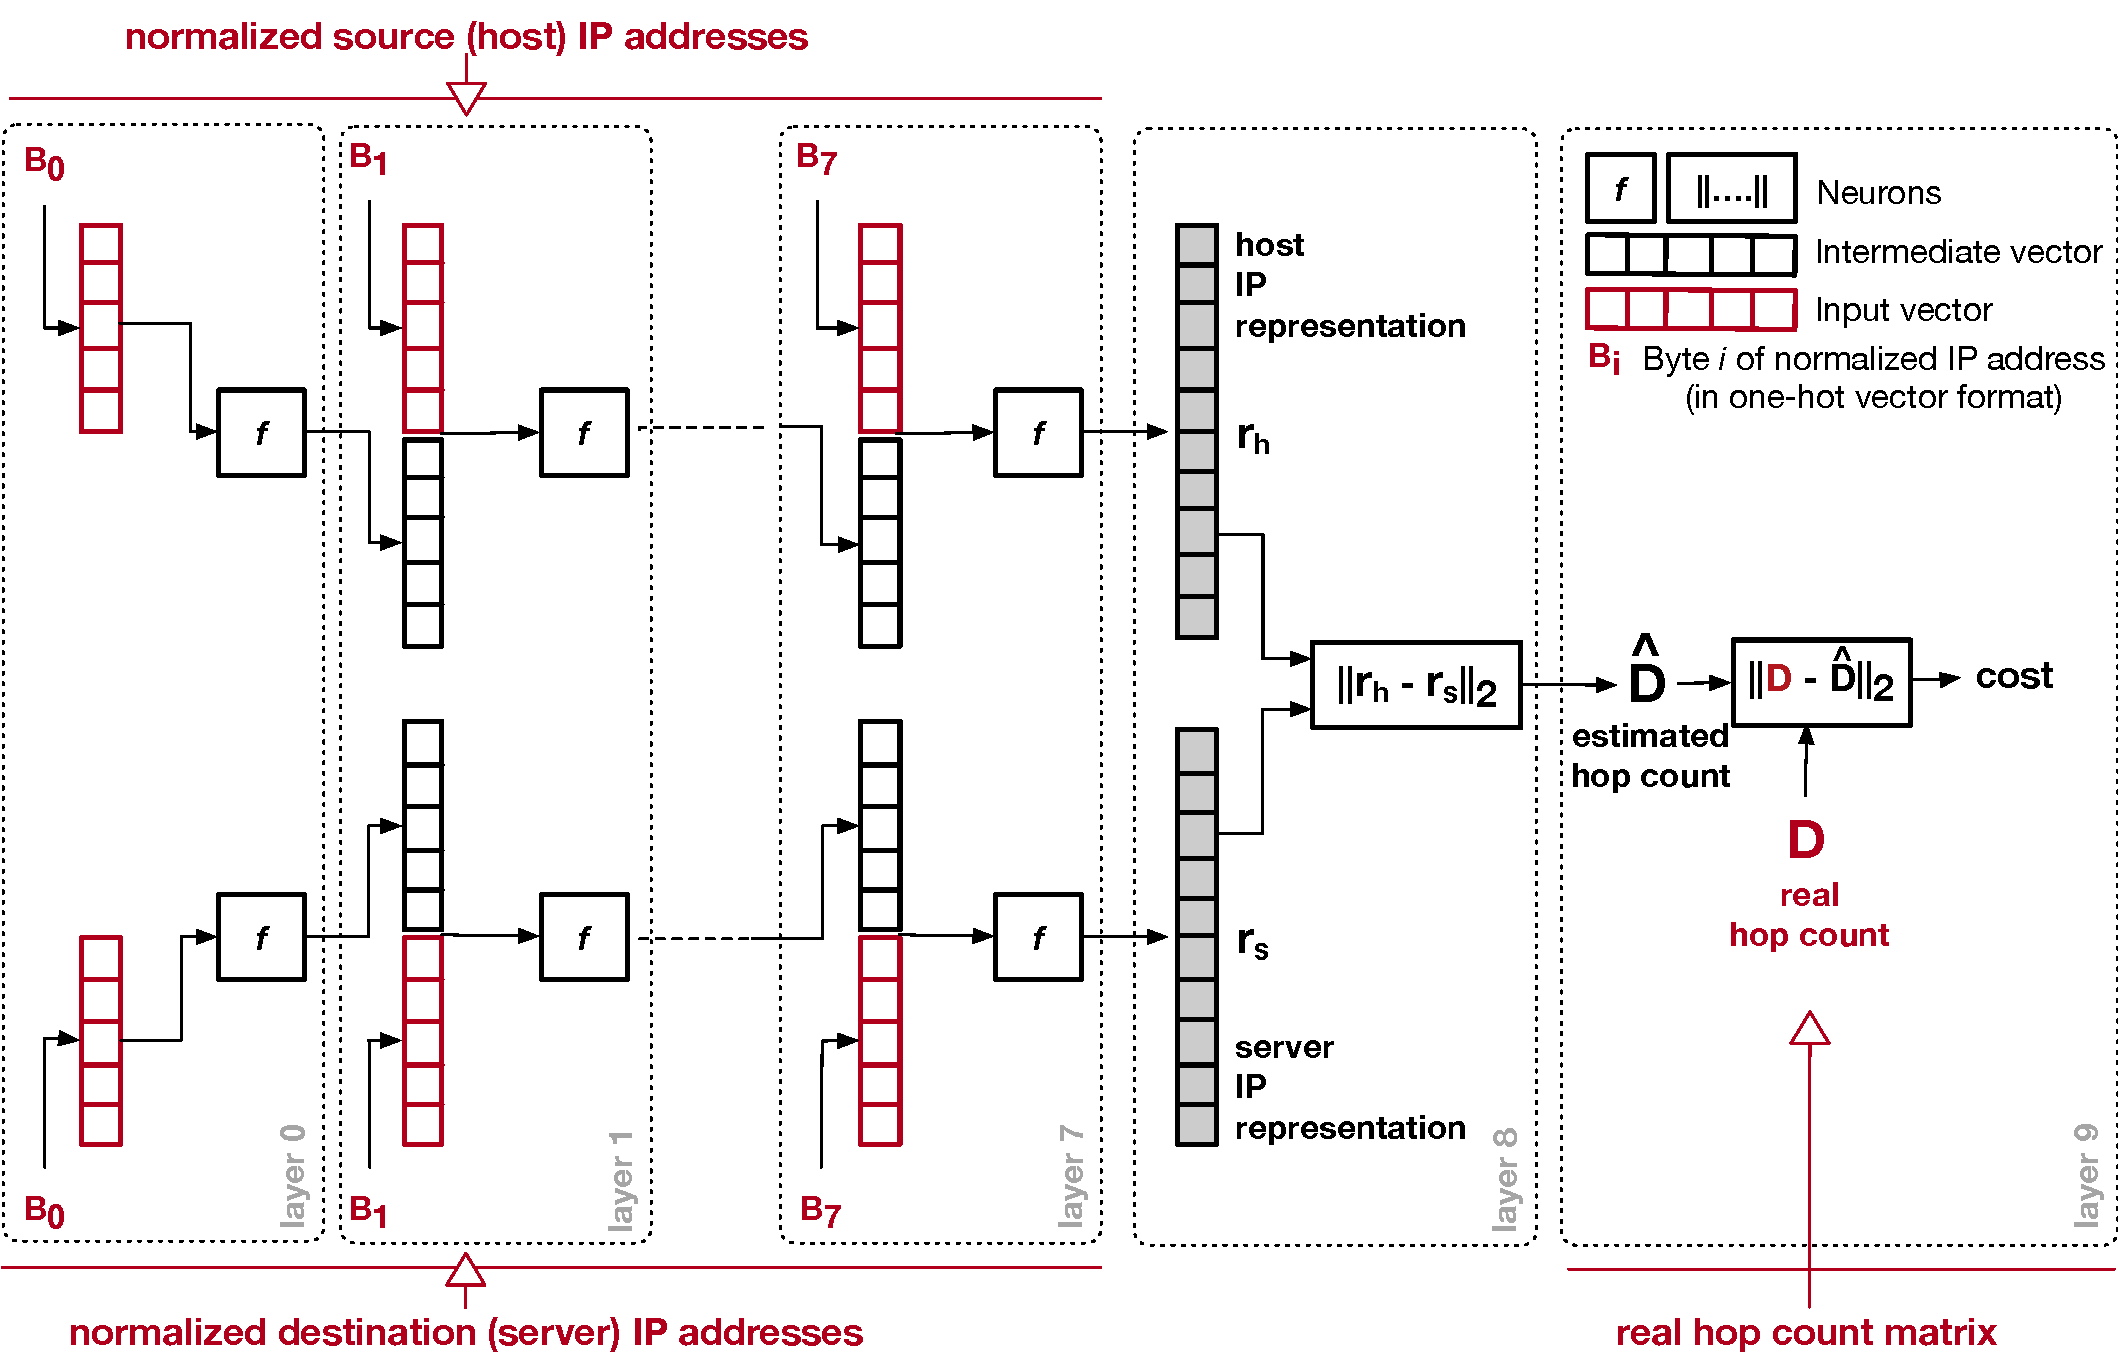
\includegraphics[width=.9\textwidth]{Graph/dip/neural-network-2}
	\end{center}

	\caption{The neural network used for training our embedding model. The first eight layers receive the normalized IP addresses as input and compute the IP representations. The ninth layer estimates the hop count between two IP addresses and the tenth layer measures the model error. Elements in red are input. For simplicity we depict the input as one-dimensional vectors (one normalized IP); in reality, all inputs are matrices.}
	\label{fig:neuralnetwork}
\end{figure*}

As shown in Figure~\ref{fig:difference}, an IP address can help learn node representations that capture the network structure. The more bytes of an IP address we know, the better we can constrain the representation we assign to it. In addition, the more significant bytes of an IP address have a higher influence on the position of the associated host relative to other hosts. Therefore, the key is to capture the sequential correlation among the bytes of an IP address. %\mingda {This insight encourages us to borrow idea from recurrent neural networks~\citep{mikolov2010recurrent}, which take sequences of input, and processes each input conditioned on the context provided by processing the previous input (\eg{}, like processing natural language), to design our network.} 

% Previous: This insight leads to our network design: a variant of recurrent neural networks~\citep{mikolov2010recurrent}, which takes sequences of input, and processes each input conditioned on the context provided by processing the previous input (\eg{}, like processing natural language).


%\textbf{Insight:} Treat the bytes of an IP address differently inside the neural network to take advantage of the hidden structural information encoded inside an IP address.



%Decision 2: Normalize IP address to encode the routable prefix information.





%Each Source IP or Destination IP is represented by a one-hot vector. Suppose there are \textit{s} Source IPs and \textit{d} Destination IPs. Each IP address will be represented by a $(s + d)$ dimension vector. If we number each IP address from 1 to $(s + d)$, then the one-hot vector $v = \{v^1, v^2, ... ,v^{(s + d)}\} $ for the $i^{th}$ is shown as following:
%\begin{equation}    {v_{i}}^u =
% \begin{cases}
%    0   &  \text{if $u != i$ } \\
%   1    &  \text{if $u == i$}
% \end{cases}                \end{equation}
%With all the $(s + d)$ one-hot vectors, an identity matrix $m$ with size $(s + d)$ could be formed. The embedding process is shown in Figure. 

%\textbf{Hop count.} This is represented by the distances between the pairs of IPs. Because %it requires two IP addresses, we propose that at each step of the algorithm we feed the IP %address to obtain an initial representation which we refine using the distance. 

\subsubsection{Network Construction}

Driven by the insight gained in the previous section, we develop \system{}, a deep neural network that computes vector representations of network hosts based on their IP addresses and the hop counts to other hosts. 
%
The design of \system{}, depicted in figure ~\ref{fig:neuralnetwork}, is similar to that of a recurrent neural network~\citep{mikolov2010recurrent}, where new data is processed in  the context provided by previous data (\eg{}, like processing natural language).
%
%Figure~\ref{fig:neuralnetwork} depicts a high-level design of \system{}. 
We explain the details below. Even though the figure and our explanation refer to the input as one-hot vectors (\eg{}, a normalized IP is represented as a vector of size 8x256=2,048), in reality the inputs are matrices (\ie{}, the number of IP addresses times 2,048). Because our hop count data (see Section~\ref{subsec:data}) is between separate end-hosts (sources) and servers (destinations) and because distances in the Internet are not always symmetric, we choose to feed the source and destination IPs separately in the neural network. %\system{} works the same when the input hop count matrix is symmetric. 

\textbf{Intermediate IP representation.} As mentioned earlier, to get the most out of the format and value of an IP address towards building a representative embedding for its host, we should treat each byte separately. The more significant bytes can provide a context for how to interpret the less significant bytes. Thus, we choose to input each byte of the normalized IP (a 256-dimension one-hot vector $B^{i\in \{0,...,7\}}_{256\times1}$) separately at each layer of the network. The input of layer $i$ is the concatenation of byte $i$ with the output of the previous layer (except for the first layer). This %\mingda{, which takes memory of preceding layers and flows previous information}:
%Suppose we want to embed each byte to dimension $d$. The output of each layer will be a vector $O^{i\in \%{1,...,8\}}_{d\times1}$. The input for each layer ($i\in \{1,...,8\}$) will be as equation \eqref{equ:input}:
\begin{align} 
\label{equ:input} 
Input=
\begin{cases}
i = 0&\parbox{.25\textwidth}{$ B^{i=0}_{256\times1}$} \\
i\in\{1,...,7\}&\parbox{.25\textwidth}{$ concat(f^{i-1}_{d\times 1},  B^{i}_{256\times1})$ } 
\end{cases}
\end{align}
where $d$ is the dimension of the final IP representation and \emph{concat} represents the vector concatenation operation.

At each layer, the activation function $f$ is given by:
%When we assign a weight $w^{i\in{\{2,...,8\}}}_{d\times(256+d) }$ ($w^{i=1}_{d\times 256 }$) and a bias $b^{i\in{1,...,8}}_{d\times1}$ for the $i^{th}$ layer, the output is represented by applying a non-linear activation function (Softsign) on the input of a layer as equation \eqref{equ:ilayer}: 
% \begin{equation} 
% \label{equ:ilayer} 
% O^{l=i}= Softsign(w^{l=i}_{d\times (256+d)}\times I^{l=i}_{(256 + d)\times 1}+b^{l=i}_{d\times1})
% \end{equation}
\begin{align} 
\label{equ:ilayer} 
f^{i}=
\begin{cases}
i = 0&\parbox{.25\textwidth}{$softsign(w^{i=0}_{d\times 256}\times B^{i=0}_{256 \times 1}+b^{i=0}_{d\times1})$} \\
\\
i\in\{1,...,7\}&\parbox{.28\textwidth}{$softsign(w^{i\in \{1,...,7\}}_{d\times (256+d)} \times concat(B^{i\in \{1,...,7\}}_{256 \times 1}, 
	f^{i-1}_{d\times 1})+b^{i\in \{1,...,7\}}_{d\times1})$ } 
\end{cases}
\end{align}
where $w^{i\in \{0,...,7\}}_{d\times (256+d)}$ are weights and $b^{i\in \{0,...,7\}}_{d\times1})$ are biases; the \emph{softsign} function is $f(x) = \frac{1}{1+|x|}$. Initially, we assign random values to all weights and zeros to all biases. We employ \emph{softsign} as the activation function for the ease of training, as \emph{softsign} is more robust to saturation compared to other popular activation functions, such as \emph{sigmoid} and \emph{tanh}. %\mingda{The weights for different layer will have different ranges. The range for the first four layers (routable layers) will be larger.												}

\textbf{Intermediate distance estimation.} We use the first eight layers of the neural network to process each of the eight bytes of the input normalized IP address. The output of the eighth layer is the intermediate vector representation for each IP address in the input data. 
%The representation is based only on the structure of an IP address. 
%The next step in the processing is to go through one more layer ($9^{th}$ layer) to improve the embedding  flexibility and accuracy in a higher dimension ($d+delta$ dimension) via adjustment of weight and bias but not normalized bytes. 
%\eqref{equ:9layer}: 
%\begin{equation} 
%\label{equ:9layer} 
%O^{i=9}= Softsign(w^{i=9}_{(d+delta)\times d}\times O^{i=8}_{d\times 1}+b^{i=9}_{(d+delta)\times1})
%\end{equation}
%Then, we could measure the error of the whole embedding in predicting the distances and refine it towards minimizing the error. 
We then use the last two layers to estimate how good the representation is.
First we compute the estimated hop counts given by the current representation using an Euclidean distance. 
%All the previous equations show the transforming for a single IP address. After applying the same transformation to all the $h$ hosts and $s$ servers, we could get 
Given two matrices $H_{h\times d}$ and $S_{s\times d}$ storing the intermediate representations for the $h$ hosts and $s$ servers separately, the estimated distance matrix is:
%\todo{Mingda: what are H and S?}Ans: Just label to distinguish the two matrices: 
%$Dist_{h\times s}$ could be described as equation \eqref{equ:distance}. The $Euclidean$ is a function created to compute the Euclidean distance of any pair of the two coordinates (rows) $r^{H_{i\in{\{1,..,h\}}}}$,  $r^{S_{i\in{\{1,..,s\}}}}$ in two matrices. 
\begin{equation} 
\label{equ:distance} 
Dist_{h\times s}=Euclidean(H_{h\times d}, S_{s\times d}) 
\end{equation}



%\todo{If I need to mention details of implementing Euclidean}

\textbf{Error reduction.} Finally, we compare the estimated hop counts with the real hop counts matrix $D_{h\times s}$ to compute the cost as the mean difference of hop-counts. 
%The goal is to minimize the difference between them. 
As the real hop count matrix is sparse, we compare only the valid entries:
\begin{equation} 
\label{equ:cost} 
Cost = \frac{\sum_{i=1}^{h} \sum_{j=1}^{s}W^{(i,j)}(||r^{H_{i\in{\{1,..,h\}}}}_{d\times1} - r^{S_{j\in{\{1,..,s\}}}}_{d\times1}|| - D^{(i,j)})}{count\, of\, non-zero\, D^{(i,j)}} 
\end{equation}
$D^{(i,j)}$ represents the value of the element at $i^{th}$ row  and $j^{th}$ column in matrix $D$. $r^{H_{i\in{\{1,..,h\}}}}_{d\times1}$ and $r^{S_{j\in{\{1,..,s\}}}}_{d\times1}$ are rows in the matrices $H_{h\times d}$ and $S_{s\times d}$, and correspond to the representation of a host or server in the embedding space. $W$ is a binary (0-1) matrix whose elements are defined as:
\begin{equation}    W^{(i,j)} =
\begin{cases}
0   &  \text{$D^{(i,j)} == 0 $} \\
1    &  \text{$D^{(i,j)} \neq 0$ } 
\end{cases}                \end{equation}
To minimize the cost, we utilize the Adam algorithm, a gradient descent based back-propagation method~\citep{kingma2014adam}, which is able to automatically tune the learning rate during the training process.


\subsection{Evaluation}
\label{dip:eval}

\subsubsection{Data and Methodology}
\label{subsec:data}

We use a large data set of network hop counts from the Ark project~\citep{ark}. The data contains hop count information from 95 geographically distributed servers to ten million IP addresses that cover all routable prefixes in the Internet. We use data collected by Ark during Jun 2015. For each IP in the data, we look up the routable prefix and normalize it using the steps in Section~\ref{dip:ipnorm}.
%
Due to the cost of monitoring a large number of IPs, not all servers have hop counts for all ten million IPs. Our hop count matrix is incomplete and contains valid entries for only 29\% of the pairs. We extract IP prefix information from Routeviews data~\citep{routeviews} and use a default value of 24 for missing prefixes.


We build a prototype for \system{} using TensorFlow. We train the neural network using several smaller data sets obtained by randomly sampling 1,000, 10,000, and 100,000 IPs from the original data and keeping only the hop counts to them. Sampling increases the sparsity of the data: less than 15\% of the entries in the smaller data sets are valid. We also vary the number of servers and the dimensionality of the embedding space. Intuitively, having fewer IPs or servers may not provide sufficient constraints to learn accurate representations and lead to an underfit model. Increasing the number of dimensions can reveal more hidden features, invisible at lower dimensions, but may lead to overfitting. Each training session has 2,500 iterations, \ie{}, passes through the neural network to update the weights and biases. We use a GPU server with four 3.5GHz quad-core Intel Xeon processors and 128GB of RAM. We generate testing sets by randomly sampling the original data and preserving the previously trained parameters for embedding arbitrary IP via its address (\eg{}, the weights and biases of each byte/layer).

%We generate testing sets by sampling the orig- inal data and making sure to preserve the parameters of training (e.g., the same number of servers or IPs).

\subsubsection{Embedding Accuracy}

\textbf{Clustering.} First, we assess how well \system{} preserves the clustering of hosts in the original IP space. For this, we group all IPs first according to their routable prefix and then at random. For each cluster we compute an embedding similarity metric, defined as the ratio between the average distance between all pairs of IP representations in the cluster and the maximum distance across all clusters. The lower the similarity value, the closer to each other the IPs of a cluster are in the embedding space. Figure~\ref{fig:clustering}(left) shows the similarity distribution for prefix-based and random clusters. Each IP representations is a 140-dimensional vector and computed after training the network using 10,000 IP addresses and 95 servers. Our embedding preserves the clustering of the original IP space well. 

\begin{figure*}[t]
	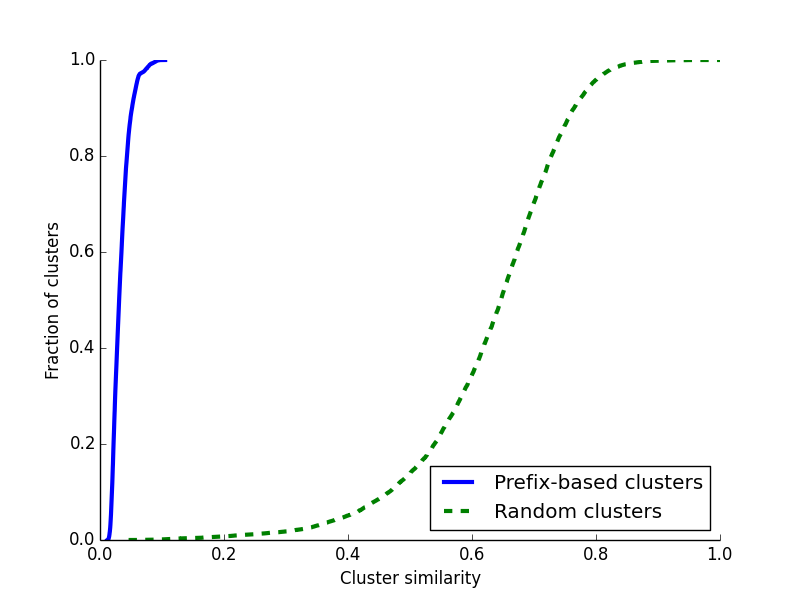
\includegraphics[width=.45\linewidth]{Graph/dip/clustering.png}
	\includegraphics[width=.45\linewidth]{Graph/dip/AbsDiffKnown12Unknown.png}
	\caption{(left) Cumulative distribution of cluster similarity, computed using IP vector representations, for prefix-based and end-host random clusters; (right) Cumulative distributions of absolute distance estimation errors for \system{}  and {\em mean}. \system{} representations preserve real-world prefix-based clustering and predict distances accurately.}
	\label{fig:clustering}
\end{figure*}

%\begin{figure}
%  \includegraphics[width=\linewidth]{AbsDiffKnown12Unknown.png}
%  \caption{Cumulative distributions of the absolute distance estimation error for \system{}  and {\em mean}.}
%  \label{fig:AbsKnown}
%\end{figure}

\textbf{Distance prediction.} To assess the quality of distance prediction, we first look at previous embedding mechanisms. Network coordinate approaches~\citep{vivaldi,gnp} are not directly comparable as they embed latencies between strategically chosen pairs of nodes, while we rely on hop count information from passively observed traffic. Eriksson~\etal{}~\citep{barford-infocom} propose a matrix factorization based algorithm to predict hop count information but first build baseline representations of the monitoring servers using an all-to-all hop count matrix. We lack complete hop count information among servers and build our embedding directly from incomplete server-to-host distances. Therefore, we compare against a {\em mean estimation approach}, where we predict a host-to-server distance as the mean of all valid distances to the same  server.

%\todo{Mingda, explain between what is the mean}
%
%\textbf{Mean estimation approach.} For the hop counts in training set between hosts and servers, we group the hop counts by servers. In each group, we calculate the mean value as the estimated hop count for the test set's same server. Meanwhile, the average value of the whole training hop counts is used  when the server in testing set is not related in training set. 


We look at how well our embedding estimates the hop count value between a host and a server. We first consider only the IP addresses used in the training process (\ie{}, {\em known IPs}). For this, we train a model using 90\% of all host-server pairs and use the remaining 10\% for testing. Figure~\ref{fig:clustering} (right) compares the absolute error between estimated and real hop count for \system{} and {\em mean} for the 10,000 IPs data set on 140 dimensions. \system{} predicts distances with a mean absolute error of around two hops (23\% mean relative error) and reduces the error of the {\em mean} estimation by almost 30\%.
%
Table~\ref{tab:abserror} presents the average absolute error and standard deviation for hop count estimation for embeddings trained with different number of hosts, servers, or dimensions. As expected, increasing the the number of IPs, servers, or the dimensionality reduces the absolute error. We also trained models with parameters outside the ranges presented in the table but found no improvement.





%\begin{figure}
%  \includegraphics[width=\linewidth]{AbsDiffKnown11Unknown.png}
%  \caption{Cumulative distributions of the absolute distance estimation error for \system{}  and {\em mean}. Log Scale}%
%  \label{fig:AbsKnown}
%\end{figure}


%\begin{figure}
%  \includegraphics[width=\linewidth]{AbsDiffKnown.png}
%  \caption{Absolute difference for known IP address}
%  \label{fig:AbsKnown}
%\end{figure}
%\begin{figure}
%  \includegraphics[width=\linewidth]{RelDiffKnown.png}
%  \caption{Relative difference for known IP address}
%  \label{fig:RelKnown}
%\end{figure}
%\begin{figure}
%  \includegraphics[width=\linewidth]{AbsDiffKnownDiffSet.png}
%  \caption{Absolute difference for various  set of servers}
%%  \label{fig:AbsKnownCluster}
%\end{figure}
%\begin{figure}
%  \includegraphics[width=\linewidth]{RelDiffKnownDiffSet.png}
%  \caption{Relative difference for various set of servers}
%  \label{fig:RelKnownCluster}
%\end{figure}
%\begin{figure}
%  \includegraphics[width=\linewidth]{AbsDiffunknown.png}
%  \caption{Absolute difference for known and unknown IP address}
%  \label{fig:Absunknown}
%\end{figure}
%\begin{figure}
%  \includegraphics[width=\linewidth]{RelDiffunknown.png}
%  \caption{Relative difference for known and unknown IP address}
%  \label{fig:Relunknown}
%\end{figure}
\iffalse
\begin{table}

		\begin{tabular}{c|c|c|c|c}
			& \textbf{\system{}} & \textbf{\system{}}& \textbf{mean} & \textbf{mean}\\
			& \textbf{known IPs} & \textbf{new IPs}& \textbf{known IPs} & \textbf{new IPs}\\
			\hline
			\multicolumn{5}{l}{\bf Number of IPs}\\
			\hline
			1,000 & 2.13690 (1.78253) & 2.88863 (2.38421) & 2.99 (2.44) & 3.27 (2.51) \\
			10,000 & 2.08812 (1.84692) & 2.71904 (2.31317) & 2.99957 (2.42138) & 3.04499 (2.43272) \\
			100,000 & abs (std) & abs (std) & abs (std) & abs (std) \\
			\hline
			\multicolumn{5}{l}{\bf Number of servers} \\
			\hline
			12 & 2.94 (2.58) & 2.95695 (2.48825) & 3.09755 (2.56616) & 2.98796 (2.55121) \\
			24 & 2.39154(2.13572) & 2.78193 (2.3314) & 2.90291 (2.36156) & 2.96651 (2.41520) \\
			48 & 2.33922 (2.04926) & 2.75361 (2.27355) & 2.99442 (2.39106) & 3.02161 (2.40399) \\
			95 & 2.08812 (1.84692) & 2.71904 (2.31317) & 2.99957 (2.42138) & 3.04499 (2.43272) \\
			\hline
			\multicolumn{5}{l}{\bf Embedding dimension} \\
			\hline
			110 & 2.27621 (1.93433) & 2.79710 (2.39204) & 2.99957 (2.42138) & 3.04499 (2.43272) \\
			140 & 2.08812 (1.84692) & 2.71904 (2.31317) & 2.99957 (2.42138) & 3.04499 (2.43272) \\
			170 & 2.18678 (1.85972) & 2.72381 (2.33045) & 2.99957 (2.42138) & 3.04499 (2.43272) \\
	\end{tabular}
	\caption{Absolute error of distance prediction when varying the number of IPs the number of servers and the embedding dimension. We show standard deviation between brackets. The default values are 10,000 IPs, 95 servers, and 140 dimensions.}
	\label{tab:abserror}
\end{table}
\fi

\begin{table}
	\centering
		\scalebox{0.9}{
		\begin{tabular}{|c|c|c|c|c|}
			\multicolumn{1}{c}{} & \multicolumn{2}{c|}{\bf \system{}} & \multicolumn{2}{c}{\textbf Mean}\\
			\cline{2-5}
			\multicolumn{1}{c}{} & \textbf{known IPs} & \textbf{new IPs}& \textbf{known IPs} & \multicolumn{1}{c}{\textbf{new IPs}}\\
			\hline
			\multicolumn{5}{l}{\bf Number of IPs}\\
			\hline
			1,000 & 2.16 (1.86) & 2.89 (2.38) & 2.99 (2.44) & 3.27 (2.51) \\
			10,000 & 2.15 (1.79) & 2.68 (2.34) & 3.00 (2.40) & 3.04 (2.43) \\
			100,000 & 2.06 (1.76) & 2.29 (2.00) & 2.98 (2.40) & 2.97 (2.40) \\
			\hline
			\multicolumn{5}{l}{\bf Number of servers} \\
			\hline
			12 & 2.79 (2.25) & 3.03 (2.47) & 3.21 (2.54) & 3.28 (2.62) \\
			24 & 2.39(2.14) & 2.60 (2.25) & 2.90 (2.36) & 2.97 (2.42) \\
			48 & 2.34 (2.05) & 2.75 (2.27) & 2.99 (2.39) & 3.02 (2.40) \\
			95 & 2.15 (1.79) & 2.68 (2.34) & 3.00 (2.40) & 3.04 (2.43) \\
			\hline
			\multicolumn{5}{l}{\bf Embedding dimension} \\
			\hline
			110 & 2.28 (1.93) & 2.80 (2.39) & 3.00 (2.42) & 3.04 (2.43) \\
			140 & 2.15 (1.79) & 2.68 (2.34) & 3.00 (2.42) & 3.04 (2.43) \\
			170 & 2.19 (1.86) & 2.72 (2.33) & 3.00 (2.42) & 3.04 (2.43) \\
			\hline
	\end{tabular}
}
   
	\caption{Absolute mean error (standard deviation between brackets) of distance prediction of \system{} and {\em mean}, for both known and new IPs, when varying the number of IPs, the number of servers and the embedding dimension. The default values are 10,000 IPs, 95 servers, and 140 dimensions.}
	\label{tab:abserror}
\end{table}



\textbf{New IPs.} An important feature of \system{} is its ability to impute hop count values to arbitrary nodes based on their IP address. %No other embedding approach is able  use domain-knowledge based methods to estimate the hop count between IPs not used in the training process, such as the average distance between known IPs in the same AS~\citep{barford-infocom}, or gaussian mixture modeling~\citep{barford-sigcomm}. Instead, \system{} relies only on the value of the IP address and the learned embedding model without any other domain knowledge. 
{\em New IPs} are IP addresses not used in the training process and that DIP has never seen before.
% Previous: which are not included in the training set. 
Figure~\ref{fig:clustering} (right) and Table~\ref{tab:abserror} show that \system{} approximates distance to new IPs with high accuracy. The distance prediction error is only around half a hop more than that for known IPs. To the best of our knowledge, DIP is the first framework to predict hop counts to arbitrary hosts based only on the value of their IP address and routable prefix and without any other domain knowledge.
%, only . %We note that our results are similar to those obtained by Eriksson~\etal~\citep{barford-infocom} after refining matrix factorization with AS information.


%\vspace{-0.5cm}
\subsection{Discussion: Limitations and Opportunities}
\label{dip:discussion}

We discuss several future applications and directions of using deep learning to understand and capture the Internet structure.

\textbf{Extensions.} An important benefit of using neural networks for learning the structure of the Internet is that they can be extended easily for other data sources. 
%
Similarly to previous embedding approaches~\citep{vivaldi,gnp}, we could use latency measurements instead of, or in addition to, hop counts. This would require simply changing the cost estimation part of the neural network (last two layers). While gathering latency measurements is expensive as it introduces traffic into the network, the ability of our approach to work with sparse data can limit the cost necessary to obtain the measurements. 

Furthermore, AS membership information could help find more accurate representations as many ASes cover limited areas in the network and provide a coarse indication of locality~\citep{barford-infocom}. To add AS membership information, we could either extend the shape of our input vectors (by adding two bytes for AS number) or adapt the cost estimation layers to use AS data in estimating error, similarly to Eriksson~\etal~\citep{barford-infocom}.

\textbf{Applications.} Building a model that accurately predicts structural properties of the Internet has several applications. Knowing the distance to remote IPs can help selecting a load balancing server or an overlay peer more efficiently and without having to perform expensive measurements. Understanding how nodes are clustered can make the transmission of video or large files faster by using close-by CDN nodes. 
%
\system{} can be a passive defense mechanism against IP spoofing attacks, where malicious users change the source IP of attack packets to avoid identification and subvert authentication. By comparing the predicted distance according to the spoofed source IP to the real distance (extracted from a packet's TTL field), one could verify whether the packet is spoofed or not~\citep{hc-filter}.  This idea inspires our next research work introduced in the next section  (Learning IP Maps for Network Spoofing Detection).  

%Furthermore, to find the true source of attack traffic, one could find the true representations of the real source and map it back to the IP space. We are currently working towards extending our modeling technique to offer such security services.


\textbf{Limitations and future work.}
Our current approach uses structural information embedded in the value of IP addresses, routing data, and distances between nodes, but does not consider the actual physical links between nodes on the Internet (\ie, the Internet physical topology). Adding topology would further constrain the embedding, since it is well known that the Internet is not a metric space and latency or hop count distances cannot always be embedded in metric spaces~\citep{vivaldi}. We plan to extend our framework using graph embedding algorithms to take advantage of physical topology information~\citep{dn-emb}.

While our preliminary experiments focused on accuracy, the performance of building an embedding model is equally important. Training a model with 100,000 addresses and 95 servers on our 16-core GPU server takes a few hours, indicating that we may need to train models incrementally when resources are constrained~\citep{bruzzone1999incremental}. For example, in a live deployment, we envision reconstructing our model every few days to capture the changes in topology triggered by the dynamic Internet. We are currently studying ways to incrementally add or update models without rebuilding from scratch.

Because our data is sparse, not even the best embedding may be able to recover all structural properties. While we show that our results are reasonably accurate, even when we have less than 15\% of all distances available, getting more data is clearly helpful~\citep{barford-infocom}. We plan to use active monitoring techniques (\eg{}, {\em traceroute}) to collect more information for the training phase. Knowing the IPs and connectivity of routers in the network would make the training data set richer and constrain the representation of end-hosts further.


%\todo{I think it is 13\% for 10,000}



\section{Learning IP Maps for Network Spoofing Detection}
\subsection{Introduction}
\label{spoof:intro}

Spoofing the source IP address of network packets is a mechanism frequently used in denial-of-service attacks~\citep{spoofing-ddos,spoofing-ps}. IP spoofing can both hide the true source of the attack, thereby subverting IP-based firewalls and authentication mechanisms, and force legitimate hosts to redirect malicious traffic, thereby amplifying the effects of the attack~\citep{github-spoofing}. In 2018 alone, IP spoofing was the vehicle for several high-profile, terabyte-size DDoS attacks~\citep{cloudflare,github-spoofing}.  

There are two types of defenses against spoofing attacks. Active methods encrypt connections~\citep{ipsec}, probe suspicious IPs~\citep{puzzles}, or mark legitimate packets with unique identifiers~\citep{spm,spi}. They come at the expense of bandwidth, latency, or computation overhead~\citep{ipsec-overhead}.
%
Passive (or map-based) defenses construct explicit offline maps between IPs and immutable structural network properties, such as paths~\citep{rbf,idpf}, neighboring networks~\citep{ingress,egress,rpf}, or hop counts~\citep{iphc} and filter packets whose header information does not match the maps.


Passive map-based defenses have little detection overhead and are less intrusive than active defenses, but pose a significant construction cost.
%
Measuring the network properties associated with each IP is a long and tedious process that requires intrusively probing other hosts, querying routing tables, or passively waiting to receive sufficient traffic~\citep{hcf}.
%
In addition, as network properties are different for every vantage point, maps computed for a location cannot be easily transferred to a different location and must be recomputed.

We propose to {\em learn a structural model (or embedding) of the Internet and use the model to predict, rather than explicitly compute, IP maps}. Learning instead of measuring network properties could significantly reduce the cost of achieving complete host IP maps while making them more general. First, training a network embedding requires only a small set of ground truth information, such as distances between IPs (\eg{}, hop counts, latencies)~\citep{vivaldi,peerwise,barford-infocom}. This reduces the amount of data necessary {\em a priori} for constructing a good map, thereby reducing the construction cost. Second, network embeddings are general and can be used to predict associations between {\em any} IP and its local network properties, even when the IP was not part of the training. %However, because many of the IP associations are learned, not measured, they may not be accurate. Learned maps may lead to less precise detection, which makes them less practical.


%. The maps are placed on AS border routers inside the network~\citep{rbf,idpf,ingress,egress,rpf} (network-based detection) or on servers at the edge~\citep{iphc} (host-based detection) and filter incoming packets whose header information does not match the maps.









%
%Building end-host maps may complement in-network spoofing mechanisms but are specific to the host on which they are constructed and difficult, if not impossible to transfer to another host.

%In this chapter, we ask the following question: how can we efficiently increase the coverage of host-based spoofing to protect {\em any} server in the Internet against attack packets spoofed with {\em any} IP address? 
%
%We identify two key contributors for the incomplete coverage of existing host-based defenses: the construction cost and specificity of IP maps.
%
%Computing the network properties associated with each IP is a long and tedious process that requires intrusively probing other hosts, querying routing tables, or passively waiting to receive sufficient traffic~\citep{hcf}.
%



%
%With {\em learned maps}, hosts do not need to compute and maintain exact mappings and could predict the associations that they do not have. In addition, a model of the Internet is general and could be used to predict maps at every host.

We study the feasibility of using network embeddings to learn IP maps for spoofing detection. Towards this goal, we present and build a learning-based spoofing detector that combines DIP, our previous deep learning based network embedding algorithm~\citep{dip,dip-ccr} and hop count filtering, and a popular host-based spoofing detection mechanism~\citep{hcf}. Hop count filtering compares the hop count information of packets arriving at a target server to the known hop count value from the packets' IP source to the target. It considers a packet spoofed if the two values do not match. 
%
Rather than build an explicit map of known IP-to-hop-count associations, we use DIP to learn a network embedding that preserves hop count distance between IPs. Using the embedding, we predict with high accuracy the hop count between any two IPs and identify when a packet is spoofed.

We analyze the coverage, accuracy, and cost of our learning-based detector. We show that learning, instead of explicitly computing IP maps, dramatically increases the detection coverage over spoofed sources and targets. Our learning-based detector needs hop count information from only around 1,000 IPs to several targets to build a model that can help detect spoofing from most of the Internet. Although, not as accurate as the original hop count filtering in detecting packets spoofed with previously known IPs (\ie{}, to which the hop count is known), ours is the first map-based detector to identify spoofing with unknown IPs (\ie{}, for which the hop count to the target is not known). It can also be used to detect spoofing to new targets, not part of the training process, with only a small loss in accuracy. In addition, learning an embedding is fast: even with almost three million hop counts from 100,000 IPs, it takes less than an hour to learn an embedding that can predict maps for any IP address.

This work brings two contributions. First, we introduce a framework to help {\em any} Internet server detect packets spoofed with {\em any} IP address without any additional measurements to that IP. This represents a major shift from previous map-based spoofing detection mechanisms, who are either restricted to specific targets or to detect packets spoofed with known IPs. Although our method does not yet achieve by itself the accuracy necessary for a real-world deployment, it nevertheless shows that learning, rather than measuring, network properties could be an important piece in the spoofing detection puzzle.

Second, our work explores the impact of deep learning in the network and security operations decision making. As AI moves beyond just being the word {\em du jour} and increasingly becomes an integral part of the network, it is important to understand the trade-offs between its cost and benefits~\citep{vern}.
%
It is precisely such a trade-off that we analyze in our work: while learning IP maps for spoofing detection can ease the task of administrators and help build complete maps much faster, it may decrease the detection accuracy. Understanding this balance can lead to better and more protected networks.

%The rest of the chapter flows as follows. In the next section, we revisit map-based spoofing detection mechanisms and reiterate the motivation for learning maps. We describe our vision for a learning-based spoofing detector in Section~\ref{sec:design}. In Section~\ref{sec:eval}, we use real world data to evaluate the trade-offs involved in introducing learning to spoofing detection. We discuss the limitations and opportunities of our work in Section~\ref{sec:discussion} and conclude in Section~\ref{sec:conclusions}.

\subsection{Towards Learned Maps for Spoofing Detection}

%Internet hosts can {\em actively} protect themselves from IP spoofing by securing their connections using private keys~\citep{ipsec}, probing suspicious IPs to check their validity~\citep{xxx}, or asking sources to send the solution to a computational puzzle before connecting~\citep{puzzles}. All these solutions are expensive to deploy and may introduce performance overhead in the form of additional network throughput and latency~\citep{ipsec-overhead}.

Map-based spoofing defense mechanisms associate IP addresses with immutable network properties that are difficult to modify by attackers. Packets that carry information (\ie{}, in headers) not matching the map are dropped. Unlike active spoofing defense methods that encrypt connections~\citep{ipsec} or probe suspicious IPs~\citep{puzzles}, map-based approaches are less intrusive and do not introduce additional traffic.
%
To be effective, map-based detection must provide {\em coverage}: given a random attacker, protect any target against attack packets spoofed with any IP address.
%

\textbf{Network maps.}
Network-based maps reside on AS border routers and pair IPs to the incoming network interface~\citep{rpf,idpf} or with keys inserted in the packet by an upstream trusted party~\citep{spm}. Such maps have the potential to provide complete coverage, if installed pervasively by {\em all} ASes. However, their deployment has been slow. Recent measurements performed by CAIDA~\citep{spoofing-state} show that around 25\% of all ASes allow spoofed traffic to traverse them. Until all networks deploy network-based detection, the Internet is susceptible to spoofing.
%
A likely cause for the incomplete coverage is the misaligned economic incentives~\citep{pam17-loops}: the cost to deploy network maps is high and supported by each AS, while the benefit is incremental and spread to the entire Internet.


%
%Host-based detection aligns the incentives by pushing the detection to the edge: hosts are responsible for building their own maps and benefit immediately from them. However, this comes at the expense of decreased coverage: detection benefits only the host of the map and is limited to packets spoofed with IPs present in the host's map.



\textbf{Host maps.}
Host-based detection aligns the incentives by pushing the onus of detection towards the edge of the network. Hosts\footnote{Throughout the chapter, we interchangeably refer to the server that deploys host-based maps as host, end-host, target, destination, or victim.}, rather than routers, build and maintain IP maps and benefit immediately from them. Most notably, several solutions build maps between IPs and hop count values to the target, relying on hop count data as a measure of the network topology~\citep{iphc,hcf}. 
Hop counts can be easily derived from the IP TTL field, whose value depends on the network infrastructure (\ie{}, every router decrements the value before forwarding the packet) and cannot be easily forged by an attacker.  

By pushing map computation to the edge, host-based maps decentralize the spoofing detection process and may see decreased coverage. 
%Host map-based mechanisms have several drawbacks that could limit their detection ability. 
First, their {\em detection is limited} to packets spoofed with IPs to which the target knows the hop count. They fail in detecting packets spoofed with IPs unknown\footnote{We consider an IP address {\em unknown} to a target if the target does not know the hop count to it. Existing host-based maps cannot detect packets spoofed with an unknown IP address.} to the target. As attackers rely on surprise and obfuscation, they often use random spoofed addresses that can be from anywhere, even from non-routable
ranges~\citep{cloudflare}. Increasing coverage by building complete maps is difficult. Passively collecting hop counts from incoming traffic is not likely to provide a large coverage~\citep{hcf}, while actively probing all IPs is expensive, intrusive, and time-consuming~\citep{ark}. 
%
Second, host maps are {\em location specific}. A map associating IPs with hop counts to a target is only useful for that target and cannot be transferred to other hosts, even if they are part of the same network.
%
%Finally, unlike many structural Internet properties, maps are {\em static}. They need to be updated when paths, routes, or hop counts change. Thus, spoofing detection needs to continually monitor path changes and update maps to reflect the current state.


\textbf{Learned host maps.}
We propose to {\em learn} IP-to-hop-count mappings, instead of extracting them from incoming packets. 
%Using a limited set of IPs and hop count information, we generate a structural model of the Internet that, given any two IP addresses, can estimate the hop count between them. Learning maps can increase host-based spoofing detection (because we can estimate hop counts to any IP) and make it more general (because our model does not depend on location). 
%How can we learn a structural model of the Internet that predicts hop counts between IPs? 
A natural solution is to first learn representations of IPs in a vector space and then estimate the distance (\ie{}, hop count) between IPs as the distance between their representations. Network embedding methods can easily compute IP representations in Euclidean spaces from a limited set of latency or hop count information~\citep{vivaldi,gnp,pic,pyxida,barford-infocom}. 
%
However, they are limited to the hosts part of the training set and cannot generate representations or hop counts for other hosts. This means that they cannot be used to estimate hop counts for, and thereby detect packets spoofed with, IP addresses unknown to a target.
%perform optimizations on few, strategic measurements or passive observations to learn vector representations. Oftentimes, this is not sufficient; they resort to out-of-band information, such as location~\citep{vivaldi} or routing~\citep{barford-infocom} data, or perform active measurements~\citep{barford-sigcomm} to impute the missing data and detect clusters or distances.

The emergence of learning frameworks that preserve structural network properties such as distances or clustering among nodes offers an alternative to build explicit host-based IP maps from passive or active measurements~\citep{dip,net-emb}. 
%
Deep learning based embeddings use several data sets, \ie, distances, routing information and host IP values, to learn IP representations. Because they learn hidden structural features encoded in a node's IP address, they could generate representations for any node, given only its IP address~\citep{dip}. In addition, deep learning algorithms are easily extensible and adaptable when new or updated data is available. 

%Deep neural networks consist of multiple layers of interconnected neurons~\citep{lecun2015deep}. A neuron aggregates multiple input values using local weights and biases, applies an activation function, and produces one or more numerical values as output. 
%
%Given a training task, one can define an objective function to evaluate the output of the entire neural network, \eg{}, prediction error. 
%
%Using gradient-based back-propagation algorithms to optimize the objective function~\citep{kingma2014adam}, neural networks automatically tune the weights and biases of each neuron to archive better performance.

Figure~\ref{fig:learnedmaps} presents a visual representation of the benefits of learning-based spoofing detection. Unlike network maps, which detect only spoofed packets traversing protected ASes (left diagram), or explicit host maps, which detect only packets spoofed with IP sources known by the host (middle diagram), learned host maps can detect packets spoofed with unknown IPs (right diagram). The host uses a learned structural model of the Internet to estimate a specific network property, \eg{} hop count information, associated with the source IP of an incoming packet and decide whether the packet is spoofed or not. In the next section, we describe a learning-based spoofing detector combining hop count filtering with the DIP network embedding framework.


\begin{figure}
	\centering
	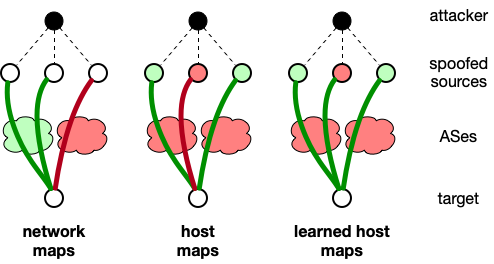
\includegraphics[width=.7\linewidth]{Graph/spoof/learnedmaps.png}
	\caption{Map-based spoofing detection. Network maps detect only spoofed packets traversing protected ASes (colored in green). Host maps detect only packets spoofed with IPs present in the map (also colored in green). Learned host maps have the ability to detect all packets because they learn missing map entries. The paths in the diagrams indicate the apparent source of the packet (the spoofed source). In reality, all packets originate from the attacker.}
	\label{fig:learnedmaps}
	\vspace{0.5cm}
\end{figure}

\subsection{Learning-Based Spoofing Detection}
\label{spoof:design}

To illustrate the benefits of a learning-based spoofing detector, we propose a prototype detection framework based on the hop count filtering method first introduced by Wang~\etal{}~\citep{hcf}.
Our prototype consists of two main components: an offline IP map learning module (to learn IP representations and estimate hop counts between IPs) and a spoofing detector (to detect spoofed traffic). We describe both modules next and study their effectiveness in the next section. 
%Building a real spoofing detection framework is a non goal of the chapter. We merely seek to understand whether a learning-based spoofing detector is a viable direction through real-world measurements.



\subsubsection{IP Map Learning}

In a previous work, we introduced DIP, a deep learning framework that uses hop count information between network host to learn an embedding of the Internet~\citep{dip}. Using a small data set of IP addresses, their prefix information, and hop counts among them, DIP computes a vector representation of each IP in a high-dimensional Euclidean space. The algorithm ensures that representations reflect hop counts between hosts: the Euclidean distance between two representations estimates the hop count between the associated IPs. We briefly describe DIP below and refer the reader to the work of ~\citet{dip, dip-ccr} for more details.


The training data for DIP includes the IP addresses and hop counts among them. The IP addresses are hierarchical sequences which contain two parts, i.e. network (routable, routing prefix) and host (local) part. For example, for a 32-bit IPv4 address 192.167.2.17/24, the number 24 means the first 24 bits form the routable prefix, which can indicate the identification of the subnet. The rest 8 bits will be the local information for this IP address within the subnet. The hop count between two IPs represents the total number of intermediate devices (e.g. routers) that a data package needs to pass. We use it as the distance between two IPs and the training objective is to estimate the hop count between two IPs. The utilized hop count matrix is actually very sparse and asymmetric. During training, we will not pre-filling any value to the matrix to avoid introducing noises. We will  measure the loss only when the hop count information exists. 

The DIP is designed to exploit the above mentioned information efficiently with a variant of recurrent neural networks to capture the structure encoded in the value of an IP address (\ie{}, network part and host part provide an implicit hierarchy of IPs). According to the definition of the network and host part, we can find it is actually more significant to use the network part expressing the structural position. However, for IP addresses, their network parts can have different sizes. The network part's size can be any value from 0 to 32 (IPv4).  Similarly, the number of bits contained in the host part varies. Hence, before feeding in the IP addresses, we will normalize them by: 1) Divide the 32 bits into network and host parts; 2) For the $n$ bits in network parts, we pad in $32-n$ 0s at the end; 3) For the $32-n$ bits in the host parts, we pad in $n$ 0s at the beginning. Then, we can get two four-byte normalized values.  

With the two four-byte values, we can convert their each byte's numerical value to a one-hot vector (256 dimensions). The reason to use one-hot vector is we think there is no relationship like natural ordering or neighboring between different values of byte. For example, there are three hosts with the second byte equalling 156, 192, 15. We cannot easily say that the first two hosts are nearer to each other compared to the third because the difference between 156 and 192 is smaller. So we would like to regard the byte value as categorical data and use one-hot vector to represent. 

By two experiments result shown in Figure 1 of \citet{dip}, we  find the more bytes for an IP address, the better we can constrain the representation of the IP. This shows the sequential information contained by the IP addresses.  So, in each layer of DIP, we feed the one-hot vector of the eight bytes from the  normalized IP separately and use the structure similar to Recurrent Neural Network to capture the sequential information. Suppose the 8 bytes are $B_i, i \in {0, ..., 7}$, where each $B$ is actually converted to a one-hot vector of 256 dimensions. The input for the first layer of DIP will be $B_0$. Via  the formula:
\begin{align} 
h_{0}=activate(W_0 \times B_0 + bias_0)
\end{align}
we can get the hidden output of the first layer. The activate function can be either $softsign$, $tanh$ or $sigmoid$. In our experiments, we use $softsign$ for an easy and efficient training.

Then, for the following layers, the hidden output of the last layer will participate into the input of the current layer. 
\begin{align} 
h_{i}=activate(W_i \times [B_i, h_{i-1}] + bias_i), i \in {1, .. , 7} 
\end{align}
The $[B_i, h_{i-1}]$ means to concatenate the current input and the last hidden state. 
Then, by the $h_7$, we can add another feedforward layer to convert the $h_7$ to $h_8$ and estimate the hop count by:
\begin{align} 
hop-count = Euclidean (h_{8,source}, h_{8, destination}),
\end{align}
which utilizes the source and destination IPs' hidden representation for estimation. During learning, the trainable parameters include the $W_i$, $bias_i$ where $i\in {0,...,7}$ and the final layer's parameters to convert $h_7$ to $h_8$. Since we think the first 4 bytes, which is the normalized network part of the IP address, are more significant for structural information. We will assign a higher initial value for the $W_i$ when $i\in {0,...,3}$ and a smaller value for the $W_i$ when $i \in {4,..,7}$. This will enhance the influence of the first four layers and weaken the influence of the second four layers. The learning will be supervised: at each iteration of the algorithm, the representations are refined towards minimizing the error between estimated hop counts (computed from the Euclidean distance between two representations) and real hop counts. 
All the previous mentioned formulas and steps are simplified version for the processes described in \citet{dip}. If you need more detailed information, please check the \citet{dip}. 

% DIP uses a variant of recurrent neural networks to capture the structure encoded in the value of an IP address (\ie{}, network part and host part provide an implicit hierarchy of IPs). To allow the most significant bits of an IP (\eg{}, the network part) to influence the final representation more than the least significant bits (\eg{}, the host part), DIP feeds the bytes of an IP address sequentially. DIP's learning is supervised: at each iteration of the algorithm, the representations are refined towards minimizing the error between estimated hop counts (computed from the Euclidean distance between two representations) and real hop counts.



The advantage of DIP compared to traditional network embedding approaches is that it incorporates structural information encoded in the value of an IP address towards learning their position in a vector space. Learning from the value of an IP address is critical for our purpose. The learned model can be used to generate representations for {\em any IP}, even if it was not part of the training set or we do not have distance information to it. This, in turn, increases the coverage of our spoofing detection. We are not limited to the information from IP maps anymore; missing associations between IPs and hop counts can be easily estimated from the learned model. In addition, embedding models are general: they can be transferred to and immediately used by other hosts, without additional retraining, thereby reducing the overall cost of achieving global detection.

Notwithstanding its advantages, DIP suffers from the same limitation as previous network embedding methods~\citep{vivaldi,gnp,pic,pyxida,barford-infocom}: Internet hop counts do not form a metric space (\eg{}, they violate the triangle inequality~\citep{peerwise}) and cannot be embedded accurately into an Euclidean space. DIP is able to predict distances between Internet nodes with a mean absolute error of 2.06 hops, after being trained on distances between around 15,000 pairs of nodes. The error increase is small (from 2.06 hops to 2.29 hops) when we consider distances to IPs not used in the training, and therefore unknown to the targets. 
%
Detecting spoofed packets based on imprecise hop count information may lead to incorrect decisions. To minimize the number of missed spoofed packets, we must allow a margin of error when comparing the estimated and real hop counts. 
%
In Section~\ref{spoof:eval}, we show that spoofing detection still works when the hop count estimations are not exact and discuss how to select the detection threshold.

\begin{figure*}[t]
	\centering
	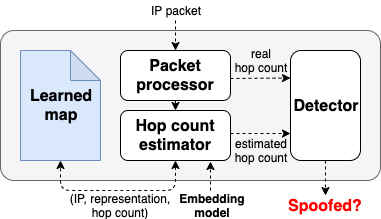
\includegraphics[width=.6\linewidth]{Graph/spoof/spoofing-detector.png}
	\caption{The learning-based spoofing detector uses an embedding of the Internet to estimate hop count information to any IP address and detect when the IP is used as the spoofed source of an attack packet.}
	\label{fig:detector}
	% \vspace{-0.5cm}
\end{figure*}

\subsubsection{Spoofing Detector}

The spoofing detector is deployed on a potential target and consists of the learned map, packet processor, hop count extractor, and detector (Figure~\ref{fig:detector}). The packet processor extracts the source IP and TTL values from an incoming packet. It then computes the hop count information from the TTL, using the algorithm described by Wang~\etal{}~\citep{iphc}. The hop count estimator uses an existing embedding model (\ie{}, built offline using IP and hop count data from legitimate packets) to compute a representation for the packet's source IP and estimate the hop count to the target. 
%
The detector compares the real and estimated hop counts to the target. If the difference between them is greater that a pre-specified threshold, we consider the packet spoofed and raise an alert.
%
To save future computation, all estimated hop counts and IP representations are saved into a cached learned map. When packets from an IP present in the map arrive at the target, we use information from the map without recomputing the hop count value.



\subsection{Evaluation}
\label{spoof:eval}

We evaluate the feasibility of learning-based spoofing detection as follows. First, we analyze what coverage we can achieve compared to detectors based on exact maps, such as hop count filtering. Second, we simulate spoofing and measure how well we detect spoofed packets under various scenarios. Finally, we look at the cost of building a detector. Table~\ref{tab:spoofing} contains a summary of our findings.

\def\arraystretch{1.5}
\setlength{\tabcolsep}{5pt}
\begin{table}[t]
	\centering
	\begin{tabular}{m{.16\linewidth}|p{.75\linewidth}}
		{\bf Method} & {\bf Description}\\
		\hline
		{\bf network maps} &  Complete coverage if all ASes deploy network maps; currently 25\% of ASes are unprotected~\citep{spoofing-state}; cost of building maps is high~\citep{pam17-loops}.\\
		\hline
		{\bf host maps} & Coverage limited to the IPs with known hop count to the host: potentially covering packets spoofed with 95\% of all IPs~\citep{hcf}, if map contains {\em all} IP addresses; maps cannot be transferred and need to be explicitly computed by each host; cost of building maps is high~\citep{hcf,ark}.\\
		\hline
		{\bf learned host maps} & Limited by the accuracy of embedding; covering packets spoofed with around 70\% of all IPs, even when the IP is unknown to the host; embedding models can be transferred and do not need to retrained; cost of building maps is low.\\
		%\hline
	\end{tabular}
	\caption{Map-based spoofing detection methods.}
	\label{tab:spoofing}
	% \vspace{-0.5cm}
\end{table}


{\bf Data.} We use a large data set of network hop counts collected by the Ark project~\citep{ark} during June 2015. The data contains hop count information from 96 geographically distributed servers to ten million IP addresses that cover all routable prefixes in the Internet. 
%
Because monitoring a large number of IPs is costly, not all servers have hop counts for all ten million IPs. Our hop count matrix is incomplete and contains entries for only 29\% of the pairs.
%
Furthermore, due to privacy issues, the last eight bits of each IP were zeroed out after collection. Although this makes the set of possible spoofed sources more general, it also helps us learn more robust models, as there are likely more servers monitoring the same /24 prefix than the same single IP address, \ie{}, the number of hop counts per IP is higher. 

It is possible that the hop counts collected by Ark are to routers on the path, rather than the end host itself. This can happen when routers, and not the target, reply to the monitoring packets. As our detection algorithm is intended for the edge of the network, training with router IPs and hop counts may bias the results. It is difficult to determine precisely which response comes from a router. To minimize the potential bias, we use a simple heuristic based on the fact that many router IPs are not part of advertised BGP prefixes. Using this heuristic, we filter out around 1.2\% of the IPs in our data.
%For each IP in the data, we extract prefix information from Routeviews~\citep{routeviews} and use a default value of 24 for missing prefixes.
%




{\bf Methodology.} We build a prototype spoofing detector using TensorFlow and Python, reimplementing the learning in DIP~\citep{dip} and hop count filtering~\citep{hcf}. We train the neural network offline using several smaller data sets obtained by randomly sampling 1,000, 10,000, and 100,000 IPs from the original data and keeping only the hop counts to them. Sampling increases the sparsity of the data: less than 15\% of the entries in the smaller data sets are valid. 
%
%We use the same training parameters as described by Li~\etal{}~\citep{dip}
%
%Li~\etal{}~\citep{dip} show that increasing the size of the training set and the dimensionality of the embedding space can increase the accuracy of hop count estimation.
%
We train our spoofing detector for 1,000 iterations on a server with four 3.5GHz quad-core Intel Xeon processors and 128GB of RAM.
%




{\bf Assumptions.} We assume a single attacker, randomly placed in the Internet, with no knowledge about network structure around the spoofing target or the spoofed IP. This means that the attacker cannot use information about hop count to the target to avoid detection. We also assume that the hop count information is static and does not change. In Section~\ref{spoof:discussion}, we discuss what happens when we relax these assumptions. 

{\bf Goals and non-goals.} Our main goal is to evaluate the feasibility of learned maps for detecting spoofed network packets and to inform future decisions of security operators or researchers. We use an existing embedding algorithm, DIP~\citep{dip} to learn hop count information between IPs, and study its interaction with hop count filtering~\citep{hcf}. A non-goal is to evaluate the DIP embedding accuracy. For a detailed study, we refer the reader to the DIP chapter~\citep{dip}, which analyzes the embedding accuracy when varying various learning parameters and in contrast to other distance prediction mechanisms.
%Our focus is thus on understanding the coverage of a learning-based spoofing detector: how likely is it to protect {\em any} target from packets spoofed with {\em any} IP address. 
\begin{figure*}[t]
	\centering
	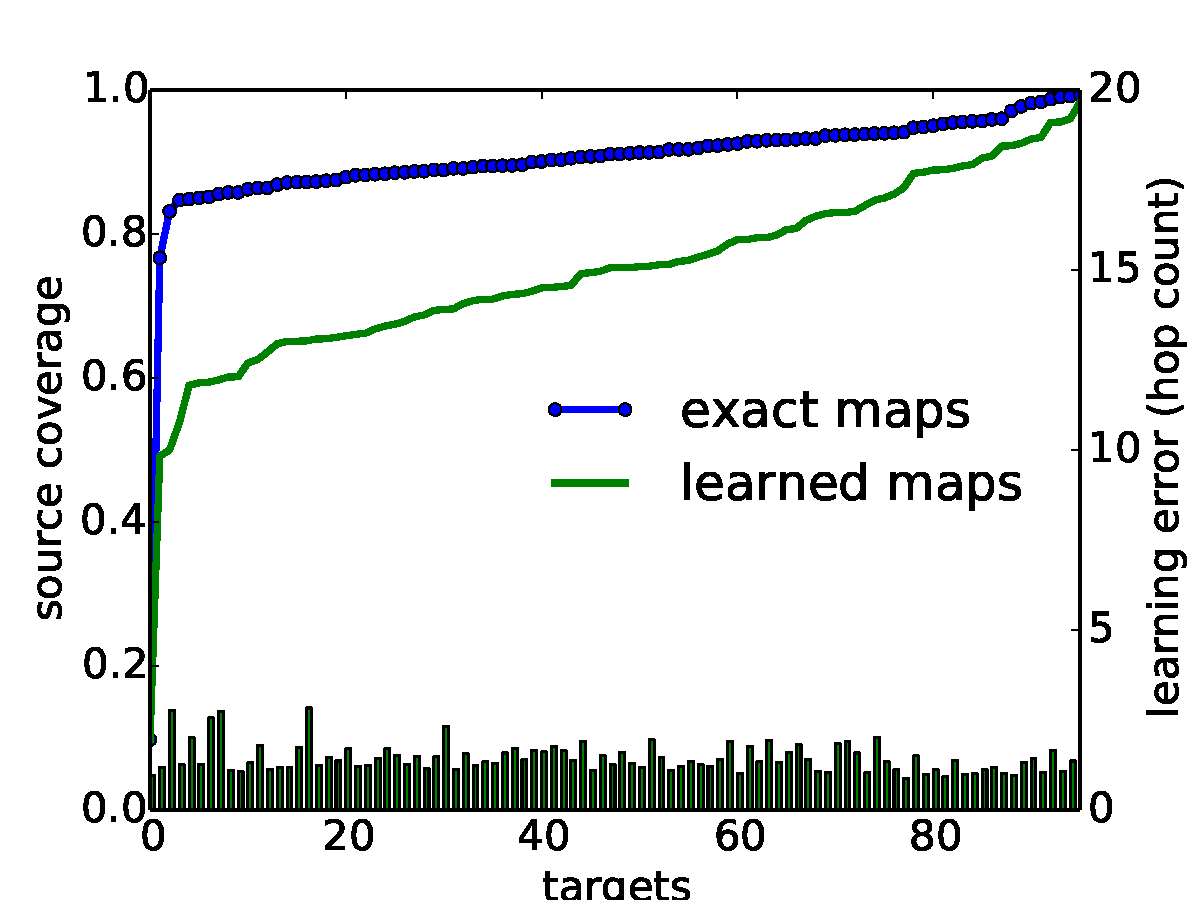
\includegraphics[width=.49\linewidth]{Graph/spoof/upperbound-upperbound-caida-jun2015-source-to-monitor-ttls-2000files-sample1000.pdf}
	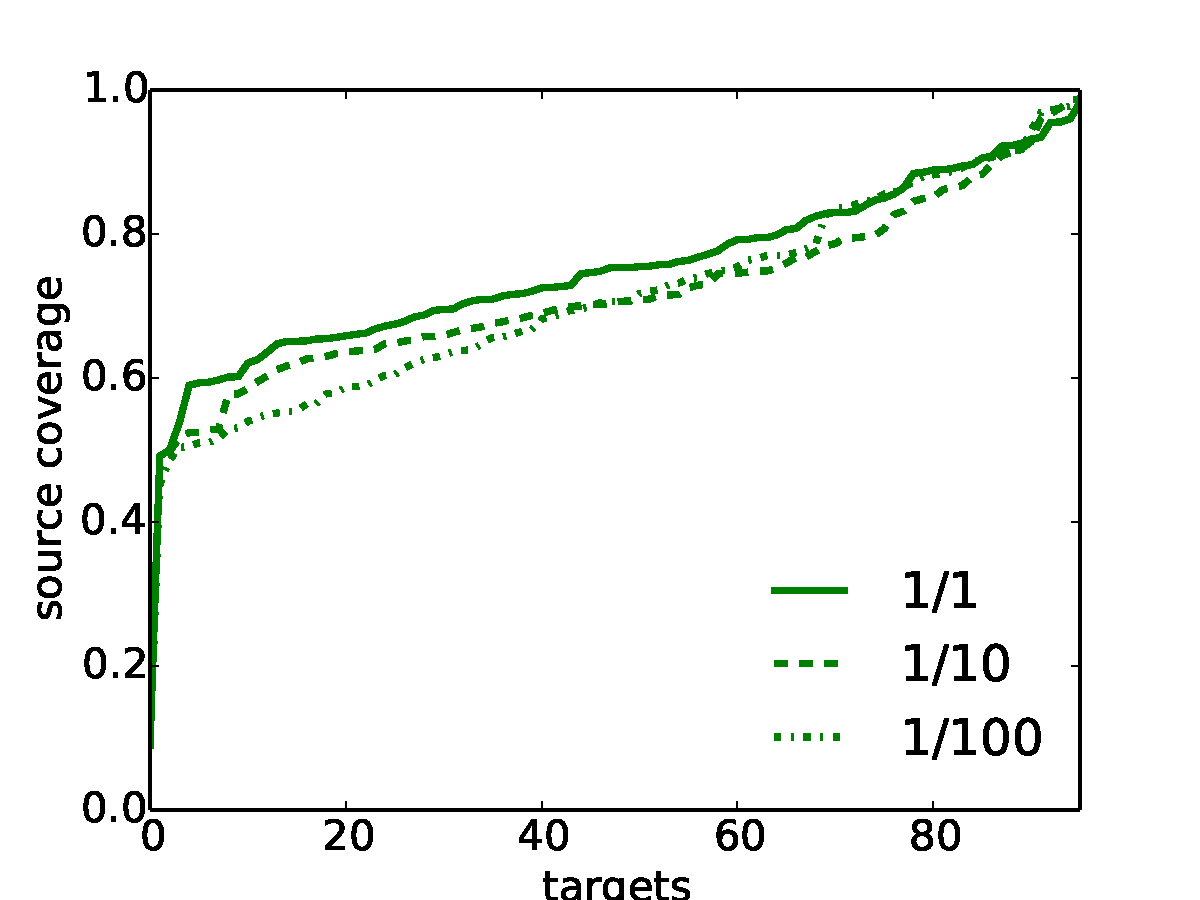
\includegraphics[width=.49\linewidth]{Graph/spoof/coverage.pdf}
	\caption{Coverage for (left) exact and learned maps for 1,000 source IP addresses, and (right) learned maps for the same sources used in training (labeled ``1/1''), ten times as many sources (``1/10''), and a hundred times as many sources (``1/100''). The bars represent the error of a learning-based spoofing detector, for each target, in hop counts. Learning-based spoofing detectors adapt well to new sources with little loss of coverage.}
	\label{fig:upperbound}
	\vspace{0.5cm}
\end{figure*}

\subsubsection{Coverage}

The limited range of hop count values (\ie{}, 0 to 255) means that no hop-count-based spoofing detector can achieve perfect detection. To understand the limits of detection, we define the {\em coverage} of each target as the expected fraction of source IPs that can be unambiguously identified when spoofed by a random attacker. In other words, the coverage represents the probability that a packet spoofed with a random IP by a random attacker is detected by the target.

{\bf Exact maps.} Before studying learning-based maps, we analyze the boundaries of what exact hop count based maps can achieve. Hop count filtering~\citep{hcf} identifies packets as spoofed when the packet hop count does not match the known hop count associated with the source address. If the attacker spoofs a packet with an IP address that has the same hop count to the target as the attacker IP, hop count filtering cannot detect the attack. 
%
To compute the coverage of exact maps, we repeatedly select a source IP at random as the attacker for each target, calculate the fraction of IPs that share the same hop count to the target as the attacker and subtract the value from 1.
%
Figure~\ref{fig:upperbound}(left) shows the distribution of coverage for all targets in our data set. We consider 1,000 IPs; results for other data sets are similar. Focus only on the line labeled {\em exact maps} for now. Most targets have a coverage of at least 0.8.

An important observation is that exact maps are not necessarily limited to detecting traffic spoofed with IPs that have communicated with the target in the past. They are efficient in detecting attacks spoofed with any IP, as long as the target knows the hop count to the IP. Oftentimes, IPs that are part of the same prefix, especially for smaller prefixes, share the same hop count to a target. Our data set already contains at most one IP per /24 prefix to ensure it does not underestimate the performance of exact maps.

{\bf Learned maps.} As described in Section~\ref{spoof:design}, learning maps introduces errors in estimating hop count values. Any learning-based spoofing detector needs to account for those errors in identifying spoofing. 
%
First, for each target, we compute the average error between real and estimated hop counts from all sources to the target. We use hop counts from 1,000 IPs to the 96 servers to learn the embedding. 
%Our training set is the same as the size of the exact maps above. 
Then, similarly to above, we select an IP at random from the 1,000 IPs in the training set as the attacker and compute the fraction of IPs whose hop count is within the estimation error of the hop count from attacker to target. We subtract this value from 1 to obtain the coverage for the learned map of each target. This captures the probability that learned maps detect packets spoofed with a random IP from a random attacker. Note that here we select an IP {\em from the training set} as the attacker to compute source coverage for known IPs and compare with exact maps. Below, we re-do the analysis for unknown IPs, that are not from the training set.
%
Figure~\ref{fig:upperbound}(left) shows that the coverage of learned maps is lower than that of exact maps when considering the same set of source IPs. On the average, a target could detect spoofed packets only 70\% of the time, compared to 90\% of the time with exact maps.

The power of learned maps lies in estimating hop counts to IPs that are {\em not} in the training set. We increase the number of source IPs to which we estimate hop counts to 10,000 and 100,000 (10, respectively 100 times more than the training set) and show the coverage in Figure~\ref{fig:upperbound}(right). Even when we increase the number of IPs 10- or 100-fold (lines labeled ``1/10'', respectively ``1/100'') compared to the training set, the coverage does not decrease much. In comparison, the coverage of exact maps for any unknown IPs {\em is 0}. Thus, learned maps offer an immense benefit when protecting against spoofing carried with IPs not known to the target.


{\bf Summary.}
IP-to-hop-count maps learned via deep learning embedding are less accurate than exact maps extracted from incoming traffic, when evaluated on IPs to which the host knows the hop count. However, learned maps dramatically outperform exact maps on unknown IPs.




\subsubsection{Accuracy}

We define the sensitivity of the detector as the fraction of detected spoofed packets out of all spoofed packets, and the specificity as the fraction of correctly identified legitimate packets out of all legitimate packets. Sensitivity (also known as recall or true positive rate) represents the probability of detecting a spoofed packet and specificity (also known as selectivity or true negative rate) captures the probability of not raising a false alert. Unlike coverage, which gives a measure of how well the detector can do for a randomly spoofed IP at any target, sensitivity and specificity measure the accuracy of the detector in a realistic scenario, given both legitimate and spoofed packets.

We set up the experiment as follows. We use the 10,000 IP data set for both training and detection. We simulate packets arriving from each of the 10,000 IPs at random and introduce spoofing with an average rate of 0.01 (one spoofed packet for every 100 packets). For each spoofed packet, we generate a fake hop count value at random from a normal distribution with a mean of 15 and standard deviation of 5. We chose these values as they match the distribution of hop counts in our data set. We measure sensitivity and specificity as averages across all targets in a specific experiment.


%We define the sensitivity of the system as the fraction of  detection on the 10,000 IP data setWe computed coverage given an estimated error threshold for each target. In reality, the host can set a different error threshold to balance the false positives and negatives. To understand how the value of the threshold can impact the detection, we define the sensitivity of a detector as the ratio of spoofed packets correctly identified to the total number of spoofed packets. A sensitivity of 1 means that we do not miss any spoofed packets, of 0 that we do not detect any. Oftentimes, identifying spoofed packets precisely is not sufficient if it comes at the expense of incorrectly detecting legitimate packets as spoofed. We define specificity as the fraction of legitimate packets out of all packets identified as legitimate. Specificity, also known as the true negative rate, measures the probability of not having a false alarm.


{\bf Varying threshold.} Figure~\ref{fig:sens}(left) shows the specificity and sensitivity as we vary the detection threshold. For a threshold of two hops, which is the average training estimation error, we obtain an overall sensitivity of around 0.75, which is consistent with the expected coverage from Figure~\ref{fig:upperbound}(left). However, a high sensitivity also results in a low specificity: while we detect most spoofed packets, we do so at the expense of tagging the majority of legitimate packets as spoofed. Modifying the detection threshold adjusts the trade-off: we find that the best balance between sensitivity and specificity is when the threshold is just above three hops. 

\begin{figure*}[t]
	\centering
	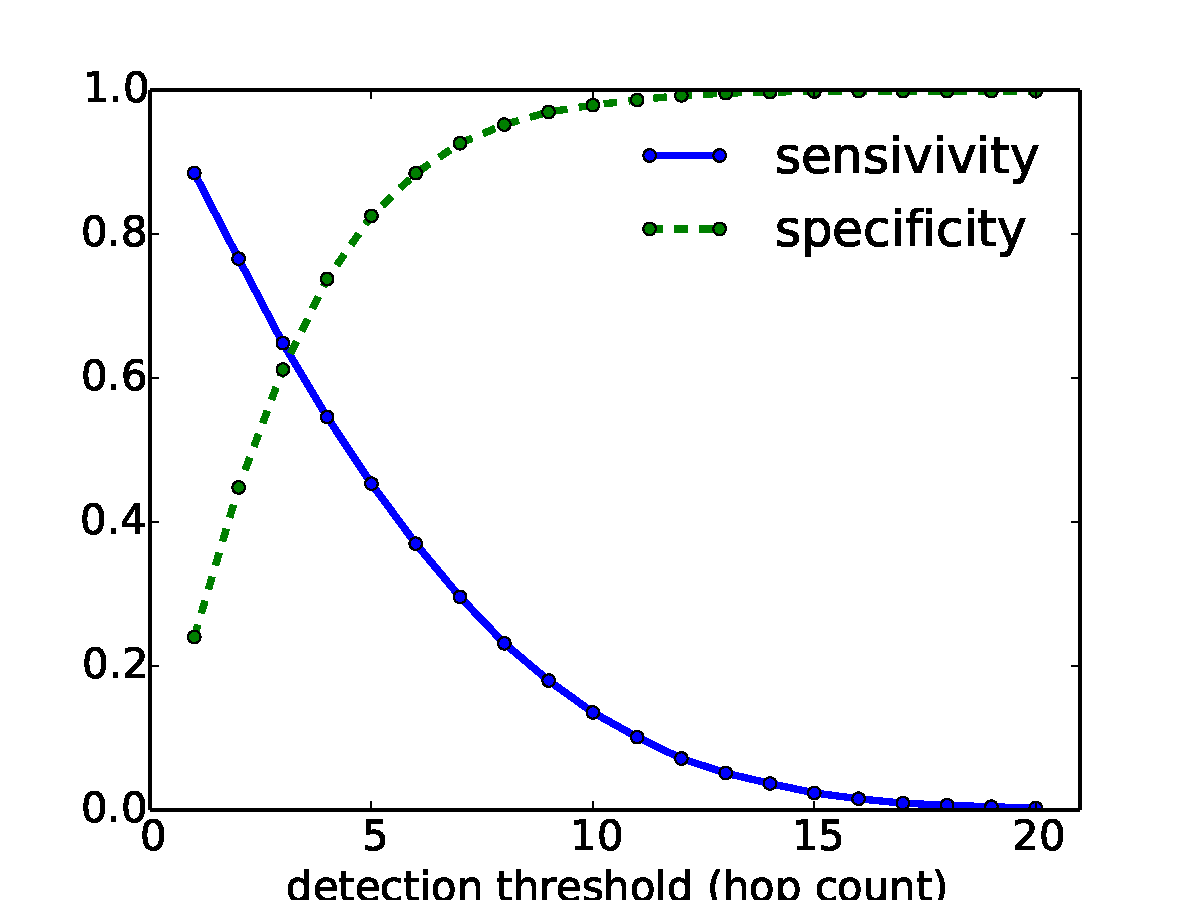
\includegraphics[width=.49\linewidth]{Graph/spoof/sens-spec-accuracy-caida-jun2015-source-to-monitor-ttls-2000files-sample10000.pdf}
	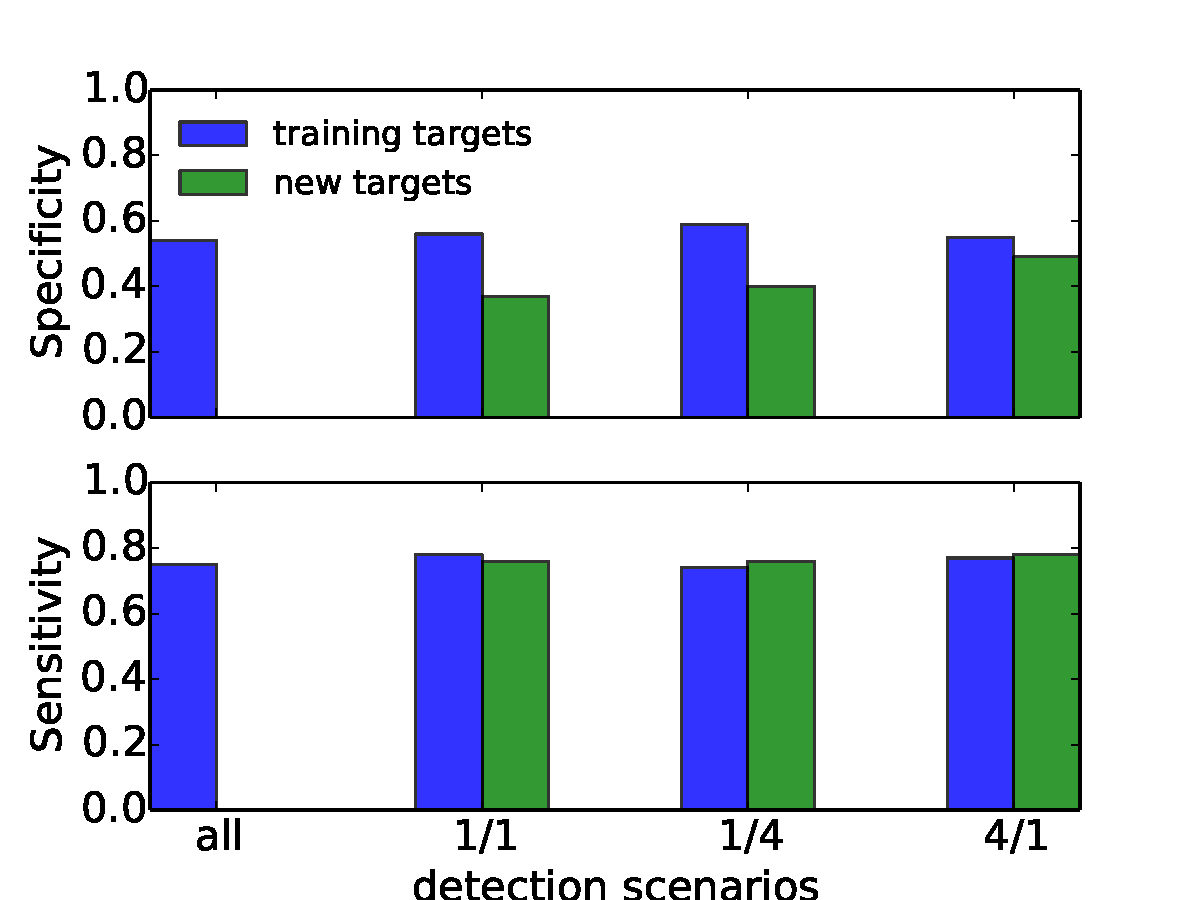
\includegraphics[width=.49\linewidth]{Graph/spoof/accuracy-bars.pdf}
	\caption{Detector accuracy under various scenarios. (left) We run detection on the  same targets used in training and vary the detection threshold; increasing the threshold reduces sensitivity and improves specificity; (right) We perform detection using both training targets and new targets not used in the training process; we set the detection threshold to two hops (the average estimation error of the model); as we vary the ratio between training and detection targets, the sensitivity for the new targets is comparable to that of the training targets, while the specificity is lower; ``all'' indicates that we perform training and detection on all targets, therefore there are no new targets.}
	\label{fig:sens}
	\vspace{0.5cm}
\end{figure*}

{\bf Summary.} Learning maps can trade-off high accuracy in detecting spoofed traffic with a high rate of false positives. This indicates that learning maps could be an important part of a bigger framework for spoofing detection, which could process the false alarms faster or dynamically adjust the detection threshold to control their rate.

\subsubsection{Model Transfer} 
\label{spoof:transfer}

To understand whether our learned model is general and can be transferred to new hosts, we split the data set into two disjoint sets, such that the targets in each set are disjoint. We train a model using only the targets in the first set and then run detection on both sets. Our goal is to understand how the detector performance for a target changes when we use a model learned for other targets. We consider three different splits: the number of targets in each set is the same (``1/1'' split), the number of training targets is four times larger (``4/1'' split) and, the training targets are four times fewer (``1/4'' split). We set the detection threshold at two hops and compute the average sensitivity and specificity for spoofing detection on each set across all splits. 

Figure~\ref{fig:sens}(right) presents the results. The sensitivity of targets not part of the training process is comparable to that of those targets used in training, showing that our models are transferable to new targets with little loss in accuracy. This reduces the cost of global deployment as new targets do not need to gather training data and build their own models. An interesting observation from Figure~\ref{fig:sens} is that the specificity of new targets is lower than for training targets: raising false alerts is more likely on hosts not part of the training.

{\bf Summary.} Maps learned at a single location are transferable to other servers in the Internet with little loss in accuracy. This is because maps are learned based on structural network properties that are the same from every vantage point and do not depend on specific locations. 


\subsubsection{Performance}

Training a representative embedding does not require significant resources. Learning a model with hop counts from 100,000 IPs to 96 servers takes about one hour on a server with four 3.5GHz quad-core Intel Xeon processors and 128GB of RAM (Table~\ref{tab:performance}). Each model takes less than 5MB of memory and thus is easily transferable over the network. Detection is fast as well. Using the same machine used for training, and given an IP packet, we are able to decide whether the packet is spoofed or not in under a millisecond. While running the detector at line speed on a network gateway instead of a powerful GPU machine may reduce these numbers, recent deep learning platforms, such as Net2Vec~\citep{net2vec}, that are able to capture and process packets at 60Gbps can make deployment easier and faster.

\begin{table}[]
	\centering
		\scalebox{0.9}{
	\begin{tabular}{l|c|c|c}
		{\bf Number of source IPs}   & 1,000 & 10,000 & 100,000 \\
		\hline
		{\bf Time to train (min)} &  1 & 6 & 58\\
		\hline
		{\bf Size of model (MB)} & 4.5 & 4.5 & 4.5\\
	\end{tabular}
}
	\caption{Performance of training for data sets containing hop count information from 96 servers to 1,000, 10,000, and 100,000 IPs. Each data set is sparse, with only about 15\% of all entries available.}
	\label{tab:performance}
	% \vspace{-0.5cm}
\end{table}

\subsection{Discussion: Limitations and Opportunities}
\label{spoof:discussion}

%We discuss several aspects related to the accuracy and deployment of our learning-based spoofing detection.

{\bf Accuracy trade-off.} Our detector trades off accuracy for generality. Low specificity may be unacceptable for many operators, who would still need to sift through alerts to identify legitimate packets incorrectly identified as spoofed. In practice, we envision that our approach works in conjunction with network-based maps and host maps built from passive measurements to offer a comprehensive and cost-efficient spoofing detection solution.

{\bf Non-metric Internet.}
Paths between Internet hosts are dictated by routing policies and AS peering agreements, and are not always shortest in terms of hop counts. Estimating the hop count between two hosts as the Euclidean distance between their embeddings does not capture the intricacies of Internet routing and may introduce errors. We are working on reducing these errors in two ways. First, we plan to introduce AS membership as an additional data set in the deep learning framework. Knowing to which AS a host belongs to can help constrain its possible positions in the embedding space. Second, we plan to add IP addresses and hop counts to routers on the path between a source and a destination. While a perfect metric embedding of Internet hop counts is impossible~\citep{peerwise}, we can reduce the learning error and better predict anomalies.

Furthermore, we are exploring non-metric embeddings. It is possible to learn structural embeddings of the Internet that estimate other network properties helpful in spoofing detection. For example, graph embeddings preserve local and remote network structure features such as first- and second-order neighbors~\citep{net-emb}. We are investigating how to use such mechanisms to devise spoofing detectors that avoid the shortcomings of hop based spoofing detection.

{\bf Dynamic Internet.}
The dynamic nature of the Internet with frequent misconfigurations, outages, or policy changes means that hop counts or IP addresses may also change~\citep{cunha, reasons}. If this happens, we may need to retrain the embedding model to reflect the updated values. A practical deployment would passively listen to incoming legitimate traffic, or selectively probe IPs from learned maps, and update existing maps to reflect new hop count values. We are currently working on how to re-train our model to learn a more accurate hop count estimation in the presence of new hop count data.

{\bf Asymmetric Internet.}
Internet routing may not always be symmetric~\citep{asym}. Due to ISP routing practices, the direct and reverse route between two nodes may be different, resulting in potentially different hop count measurements between the same pair of nodes. Because we compute hop count information from TTL values decremented exclusively by routers on the {\em direct} path between source IPs and targets, our detection is not impaired by the routing asymmetry.

{\bf Bootstrapping.} Learning a representative structural model of the Internet requires hop count measurements from many vantage points. Not all enterprises have access to many geographically distributed monitors to collect hop count data for the initial model training. There are two possibilities to generate learned maps in such scenarios. First, one could use third-party measurement data, such as that provided by CAIDA~\citep{ark}, to train a descriptive model and generate learned maps. 
%Because we use deep learning to train models, one can easily incorporate new data sources (\eg{}, AS membership information) by adding new layers or neurons. 
Second, an enterprise could deploy a model already trained in another location. As we showed in Section~\ref{spoof:transfer}, our models are transferable with little loss in accuracy. 


{\bf Attack types.}
We assumed a spoofing attack carried by a random attacker without any knowledge of the network topology. In reality, some attackers may be able to obtain information about the network that could help subvert the defense. For example, if an attacker controls multiple bots, it can send the attack from the bots that have a more popular hop count value to the target. This maximizes the likelihood of passing by our filter as there are more IP addresses with which to spoof the source.
%
Furthermore, if the attacker learns the hop count between the spoofed IP and the target, it can also spoof the TTL field of the attack packets, inserting a value that corresponds to the learned hop count. In this case, no hop count filtering can detect the attack. To learn the hop count between two arbitrary hosts, one can use DIP~\citep{dip}, the same framework we employ, or the algorithm described by Barford~\etal{}~\citep{barford-infocom}. However, both mechanisms require coordination and control of multiple geographically distributed servers, available only to more complex attackers.



\section{Conclusion}
\label{dip:conclusions}

We used deep learning to learn vector representations for nodes in the Internet based on their IP address, routing information, and a sparse hop count distance matrix. Deep learning helps uncover hidden features in the input data and recover structural properties of the Internet, such as node clusters or distances between nodes. Our experiments on a large real-world data set show that our embeddings can recover most distances, even to arbitrary hosts, with two hops absolute error, even when the training data is sparse. 
Using the deep learning framework in network spoofing detection, we found the learning-based network coordinate system (DIP) could dramatically increase the detection coverage. For any Internet server's received packets spoofed with any IP address, the DIP-based spoofing detection mechanism could determine whether the packets are spoofed or not with acceptable accuracy.  
%\todo{I think it is 13\% for 10,000}




